% 使用默认的 beamer 文档类
\documentclass{beamer}
%%%%%%%%%%%%%%%%%%%%%%%%%%%%%%%%%%%%%%%%
%%%%%% 演示文稿样式
% 支持中文
\usepackage{ctex}
% 适应中文, 首行缩进
\usepackage{indentfirst}
% 设置缩进 2 个字符
\setlength{\parindent}{2em}
% 字体修改支持
\usepackage{fontspec}
% 添加信息栏, 必须放在 usetheme 之前
% \useoutertheme{infolines}
% 规定 theme采用
\usetheme{Madrid}
% 规定颜色主题采用
\usecolortheme{default}
% 删去底部导航图标
% \setbeamertemplate{navigation symbols}{}
%%%%%%%%%%%%%%%%%%%%%%%%%%%%%%%%%%%%%%%%
%%%%%%列表样式
% 允许使用有序列表
\usepackage{enumerate}
%%%%%%%%%%%%%%%%%%%%%%%%%%%%%%%%%%%%%%%%
%%%%%%浮动体样式
% 浮动体不越过section
\usepackage[section]{placeins}
% 设置列表缩进
\usepackage[shortlabels]{enumitem}
% 三线表宏包
\usepackage{booktabs}
% 设置表格的列格式
\usepackage{array}
% 插图
\usepackage{graphicx}
% 浮动体宏包 可禁用浮动效果
\usepackage{float}
% 支持 beamer 为图片编号
\setbeamertemplate{caption}[numbered]
%%%%%%%%%%%%%%%%%%%%%%%%%%%%%%%%%%%%%%%%
%%%%%%代码样式
% 代码样式
% 设置等宽的代码字体
\usepackage{url}
% 建议这个: (linux?)
% \setmonofont{IBM Plex Mono}
% win 用户请
\setmonofont{Courier New}
%%%%%%%%%%%%%%%%%%%%%%%%%%%%%%%%%%%%%%%%
% 自定义命令及其他
% block, alertblock, exampleblock

%%%%%%%%%%%%%%%%%%%%%%%%%%%%%%%%%%%%%%%%
% 文档备注
% 第二部分实验总结报告
% 截止 2021-6-8 下午11:55
% 允许重新提交的次数: 无限制
% 指导:
% 每位同学对07-12共5次实验进行总结,形成PPT格式报告.
% 报告内容包括但不限于: 实验过程(简), 实验心得, 遇到的问题,
% 与理论课联系, 对实验设置的建议等等.
% PPT报告时间不超过10分钟.
% 所有同学都需要提交PPT,该评分计入总成绩.

%%%%%%%%%%%%%%%%%%%%%%%%%%%%%%%%%%%%%%%%
% 文档信息
\title{计算机网络实验 07-12 总结}
\author{chuan-325}
\institute[UCAS]{University of Chinese Academy of Sciences}

%%%%%%%%%%%%%%%%%%%%%%%%%%%%%%%%%%%%%%%%
\begin{document}
\section*{封面}
% 封面页
\begin{frame}
    \maketitle
\end{frame}

\begin{frame}{索引}
    \tableofcontents
\end{frame}
%%%%%%%%%%%%%%%%%%%%%%%%%%%%%%%%%%%%%%%%
%%%%%% 实验 7
\section{实验 7: 数据包队列管理实验}
% 节标题
\begin{frame}
    \sectionpage
\end{frame}

% 实验过程
\begin{frame}{实验过程}{实验 7: 数据包队列管理实验}
    \begin{block}{主要内容}
        1. 复现 bufferbloat 问题, 调研队列大小对传输中各个指标的影响;\\
        2. 使用不同的算法解决 bufferbloat 问题,
        并复现论文中对不同算法及动态带宽下的RTT测量结果.
    \end{block}
\end{frame}

% 实验结果展示: 复现
\begin{frame}{复现 bufferbloat}{实验 7: 数据包队列管理实验}
    \begin{figure}[h]
        \centering % 居中显示
        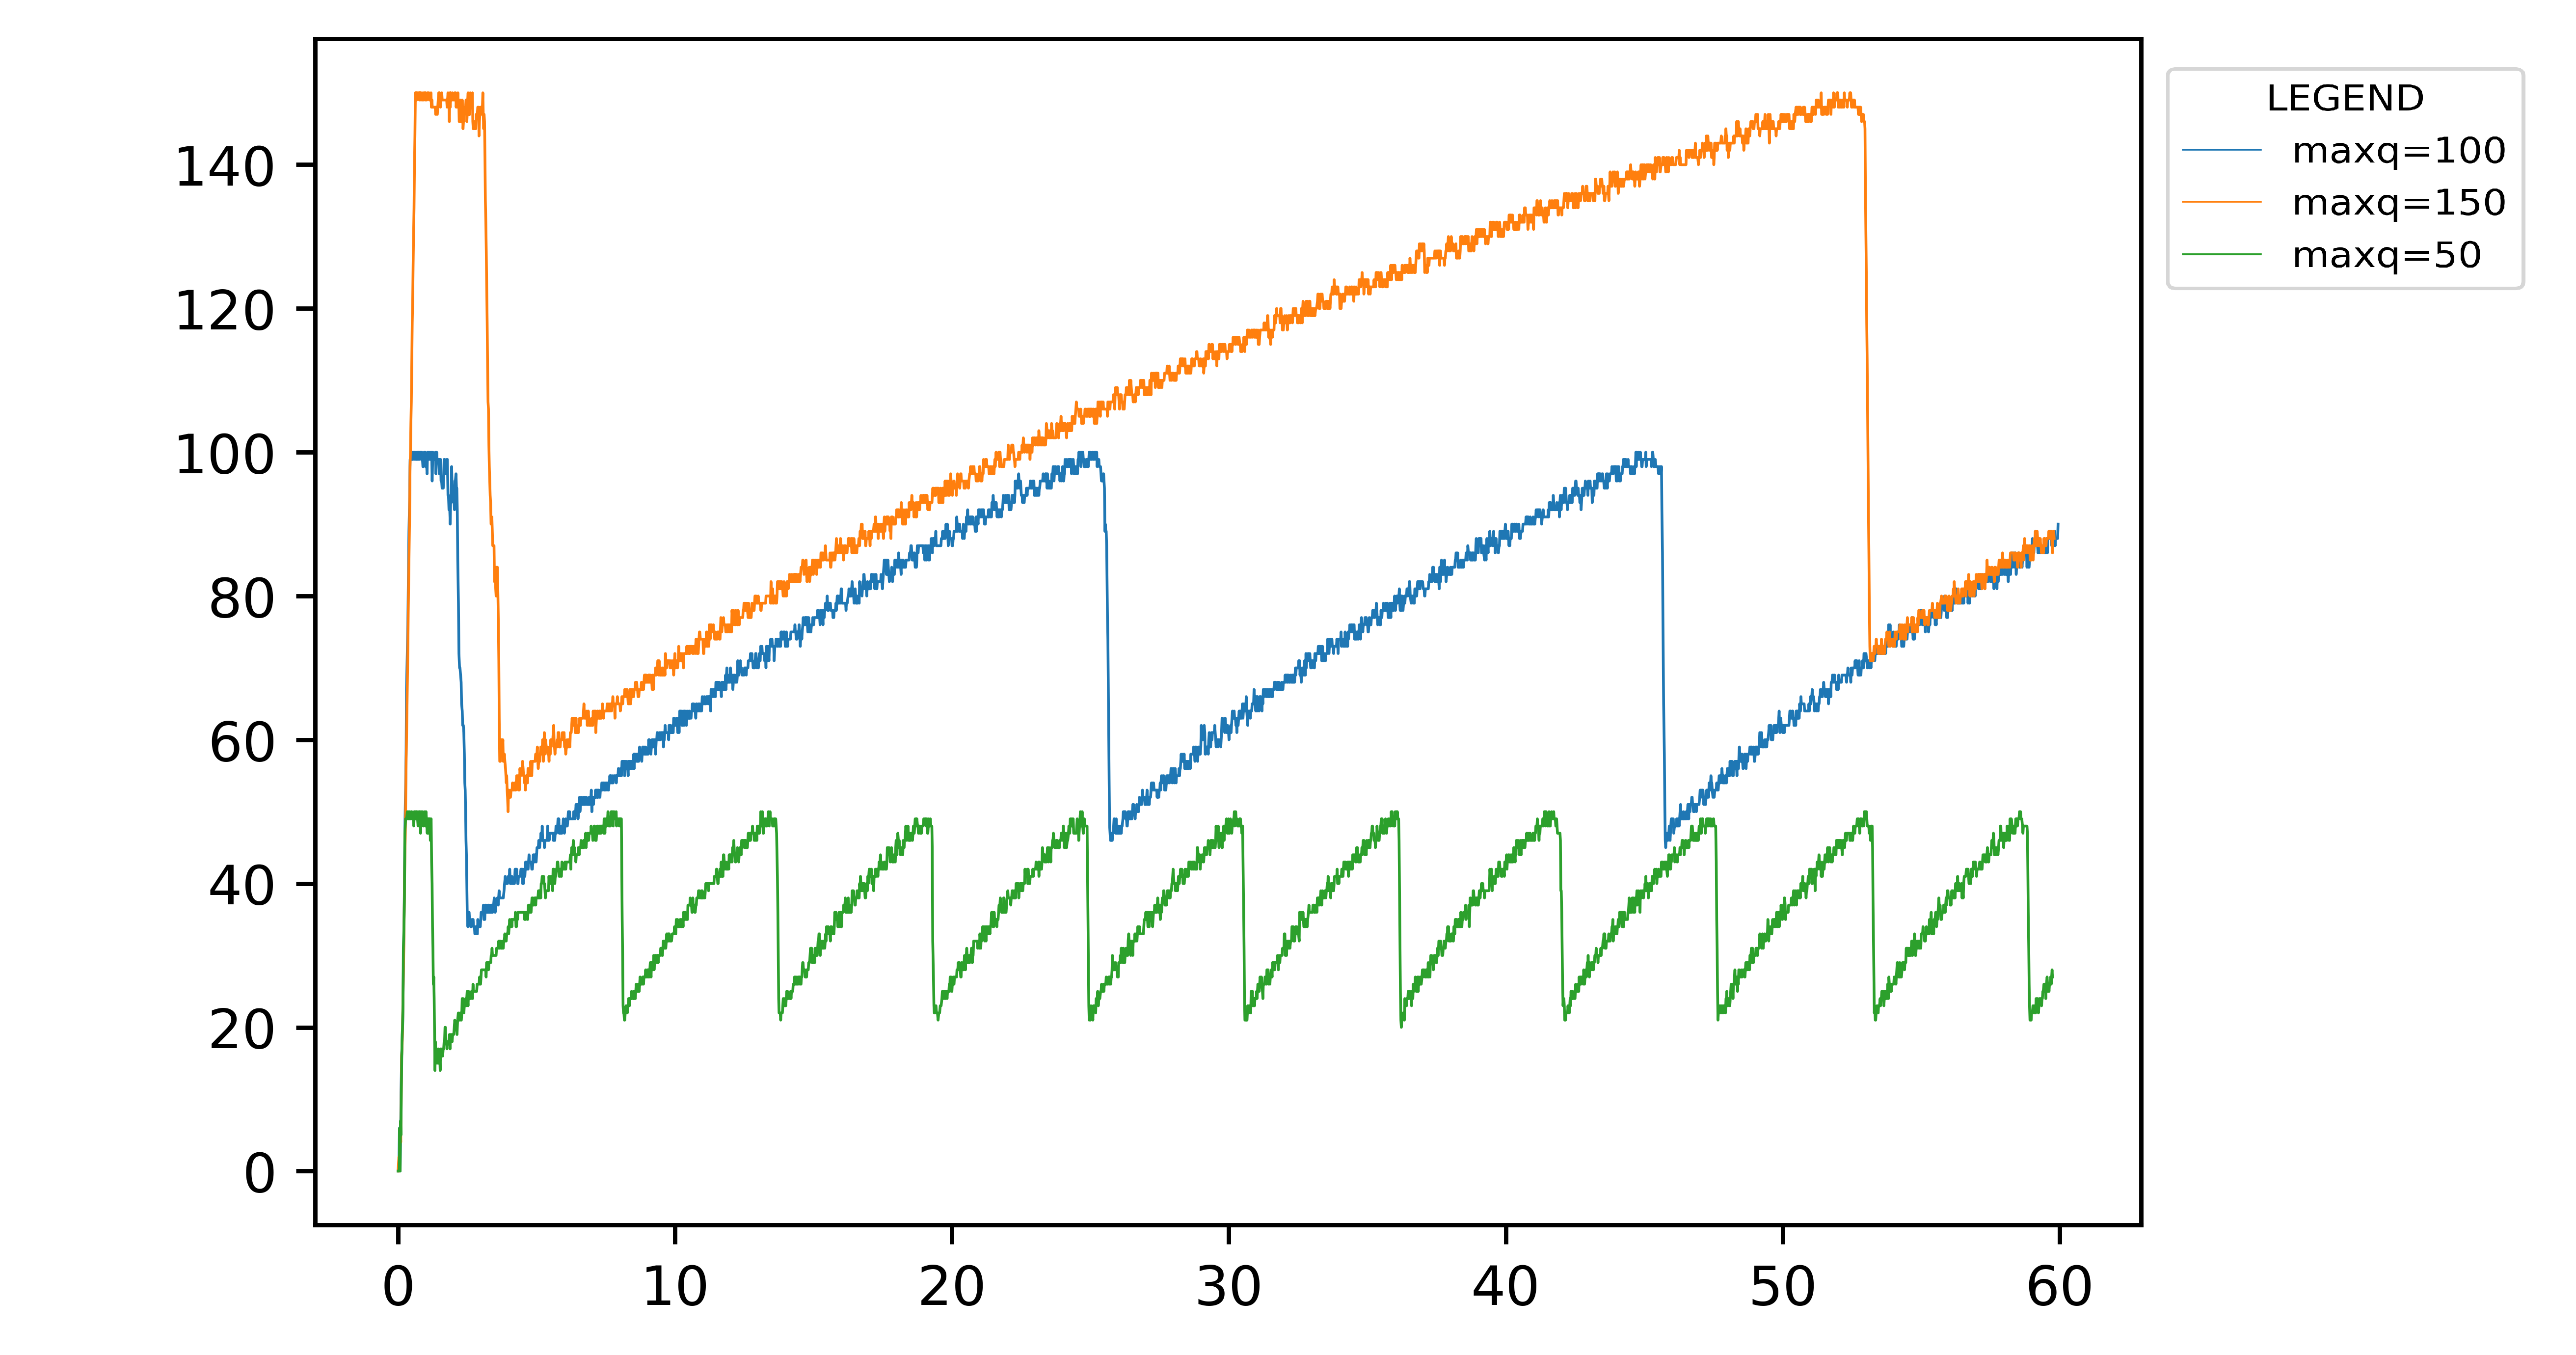
\includegraphics[width=280pt]{
            ../lab-07-pktq/readme.assets/rp-qlen.png}
        \caption{qlen 值随时间 (单位: s) 变化曲线图} % 标题
    \end{figure}
\end{frame}
\begin{frame}{复现 bufferbloat}{实验 7: 数据包队列管理实验}
    \begin{figure}[h]
        \centering % 居中显示
        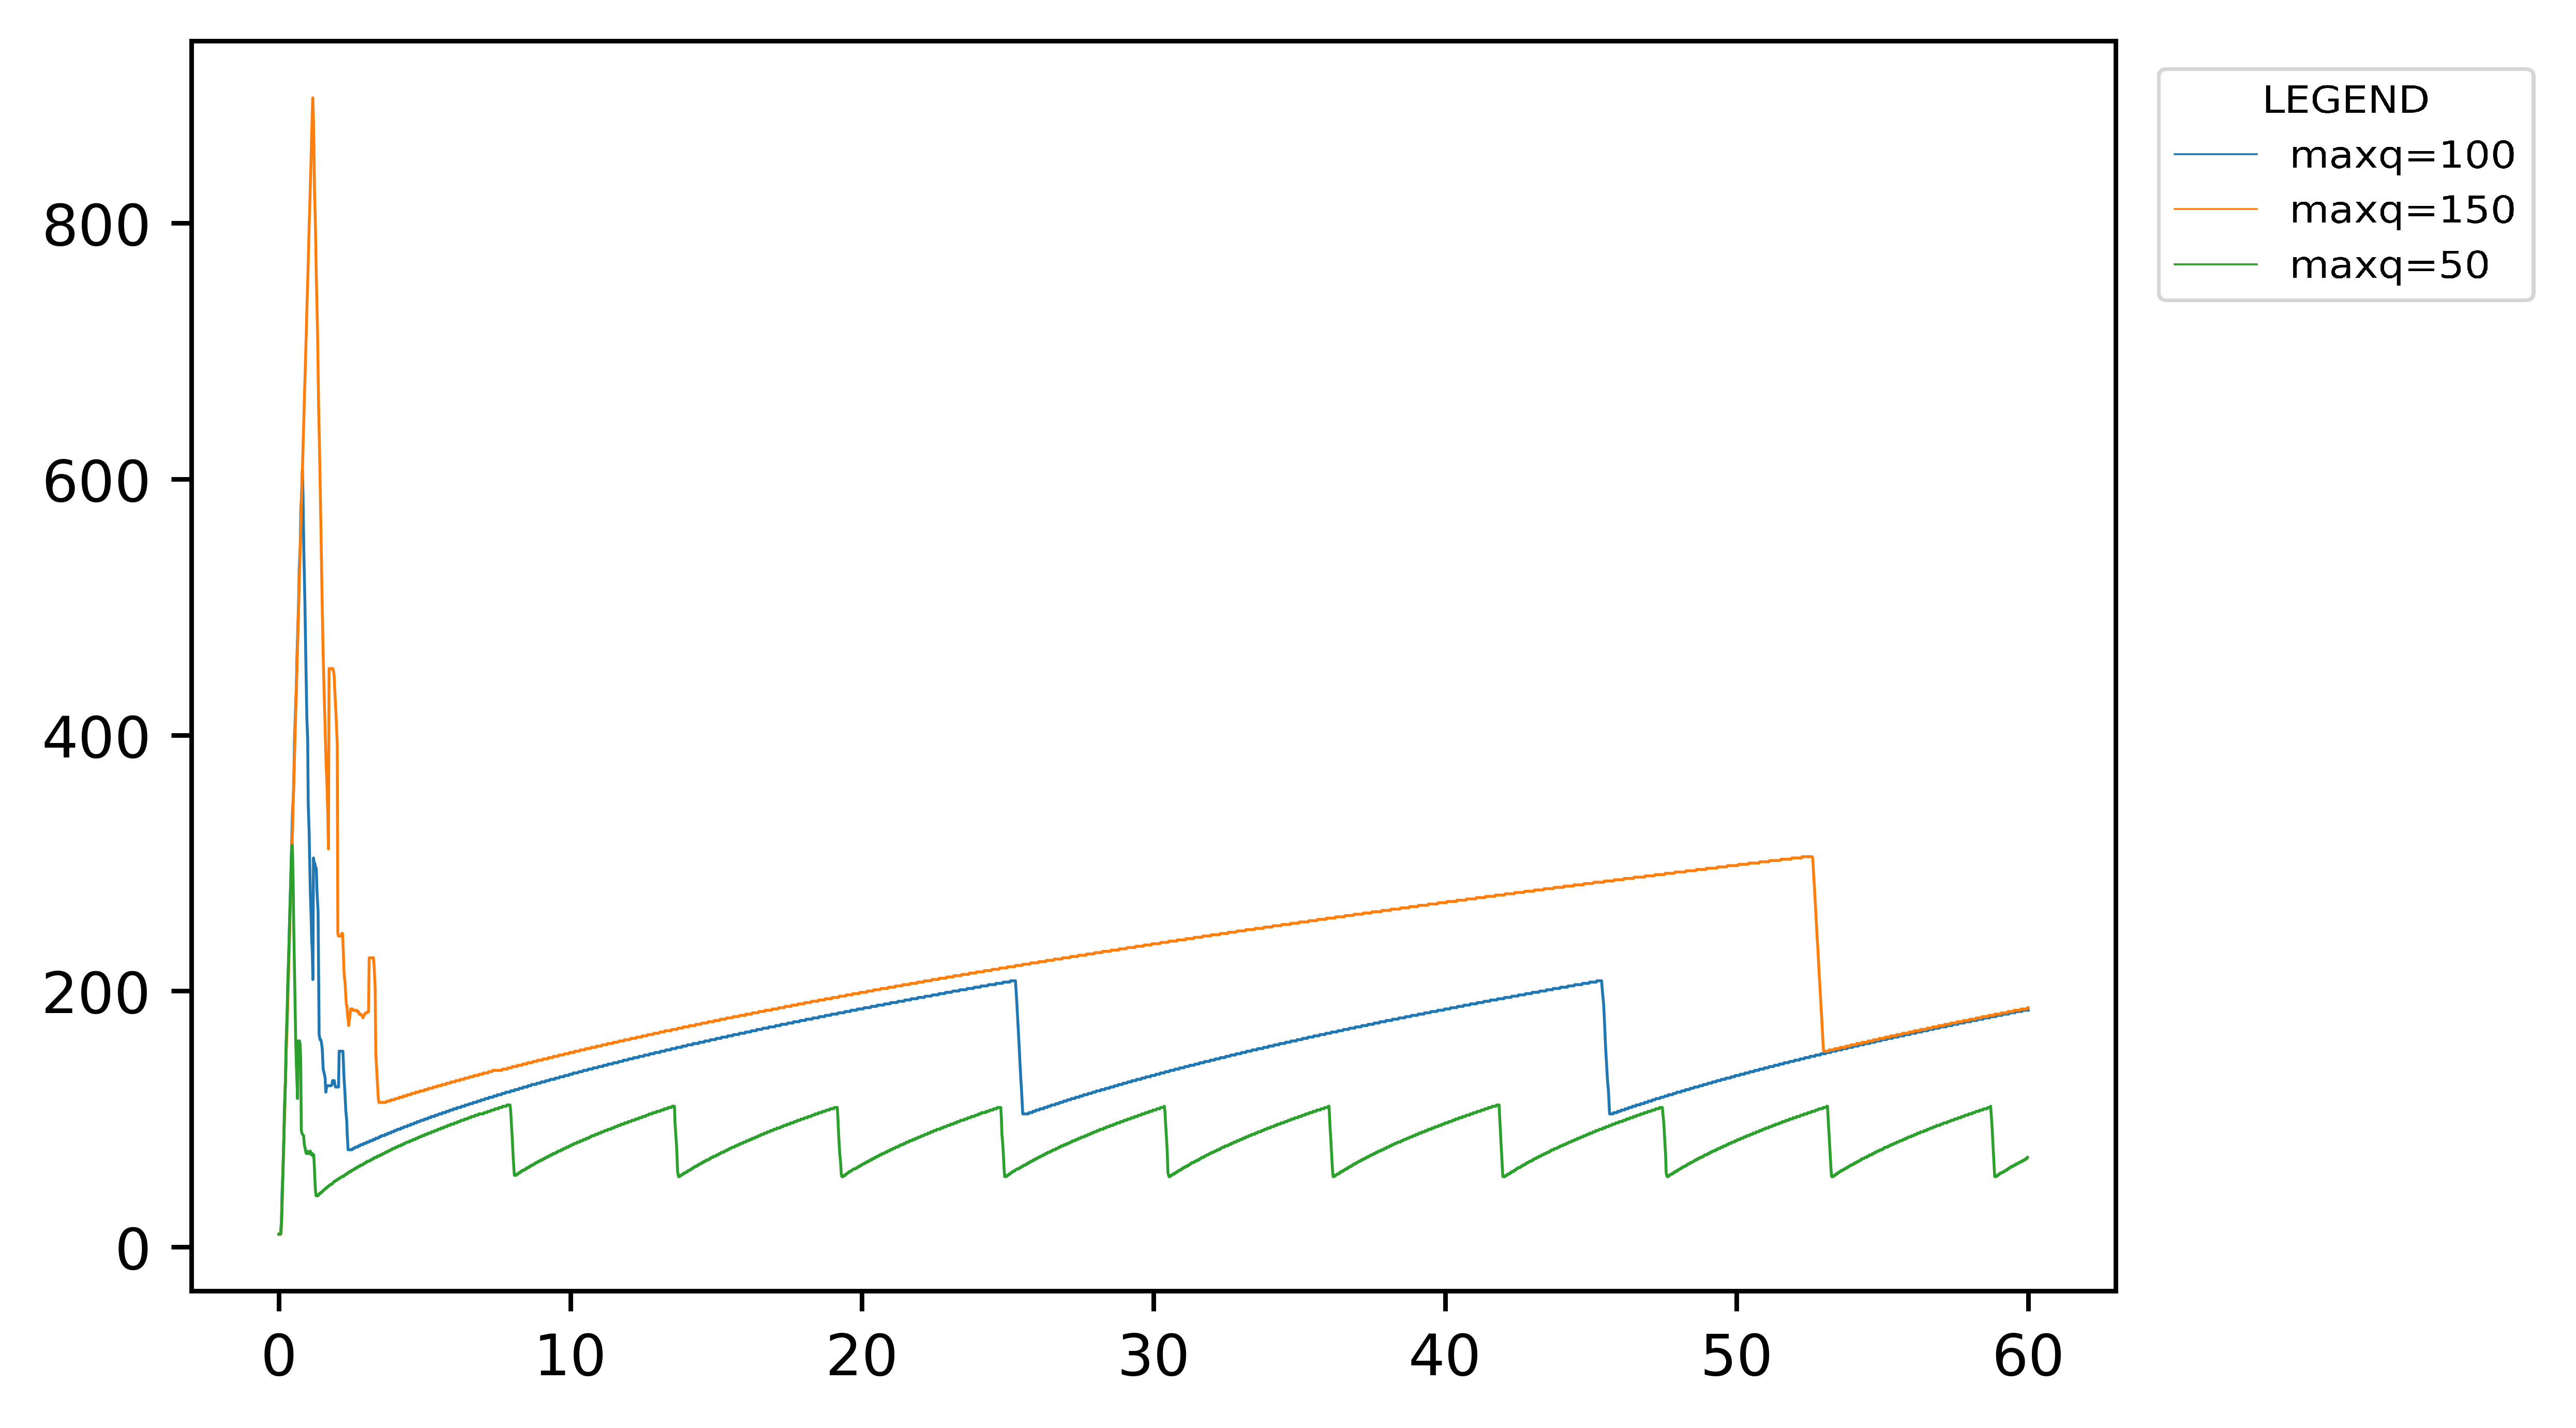
\includegraphics[width=280pt]{
            ../lab-07-pktq/readme.assets/rp-cwnd.png}
        \caption{cwnd 值随时间 (单位: s) 变化曲线图} % 标题
    \end{figure}
\end{frame}
\begin{frame}{复现 bufferbloat}{实验 7: 数据包队列管理实验}
    \begin{figure}[h]
        \centering % 居中显示
        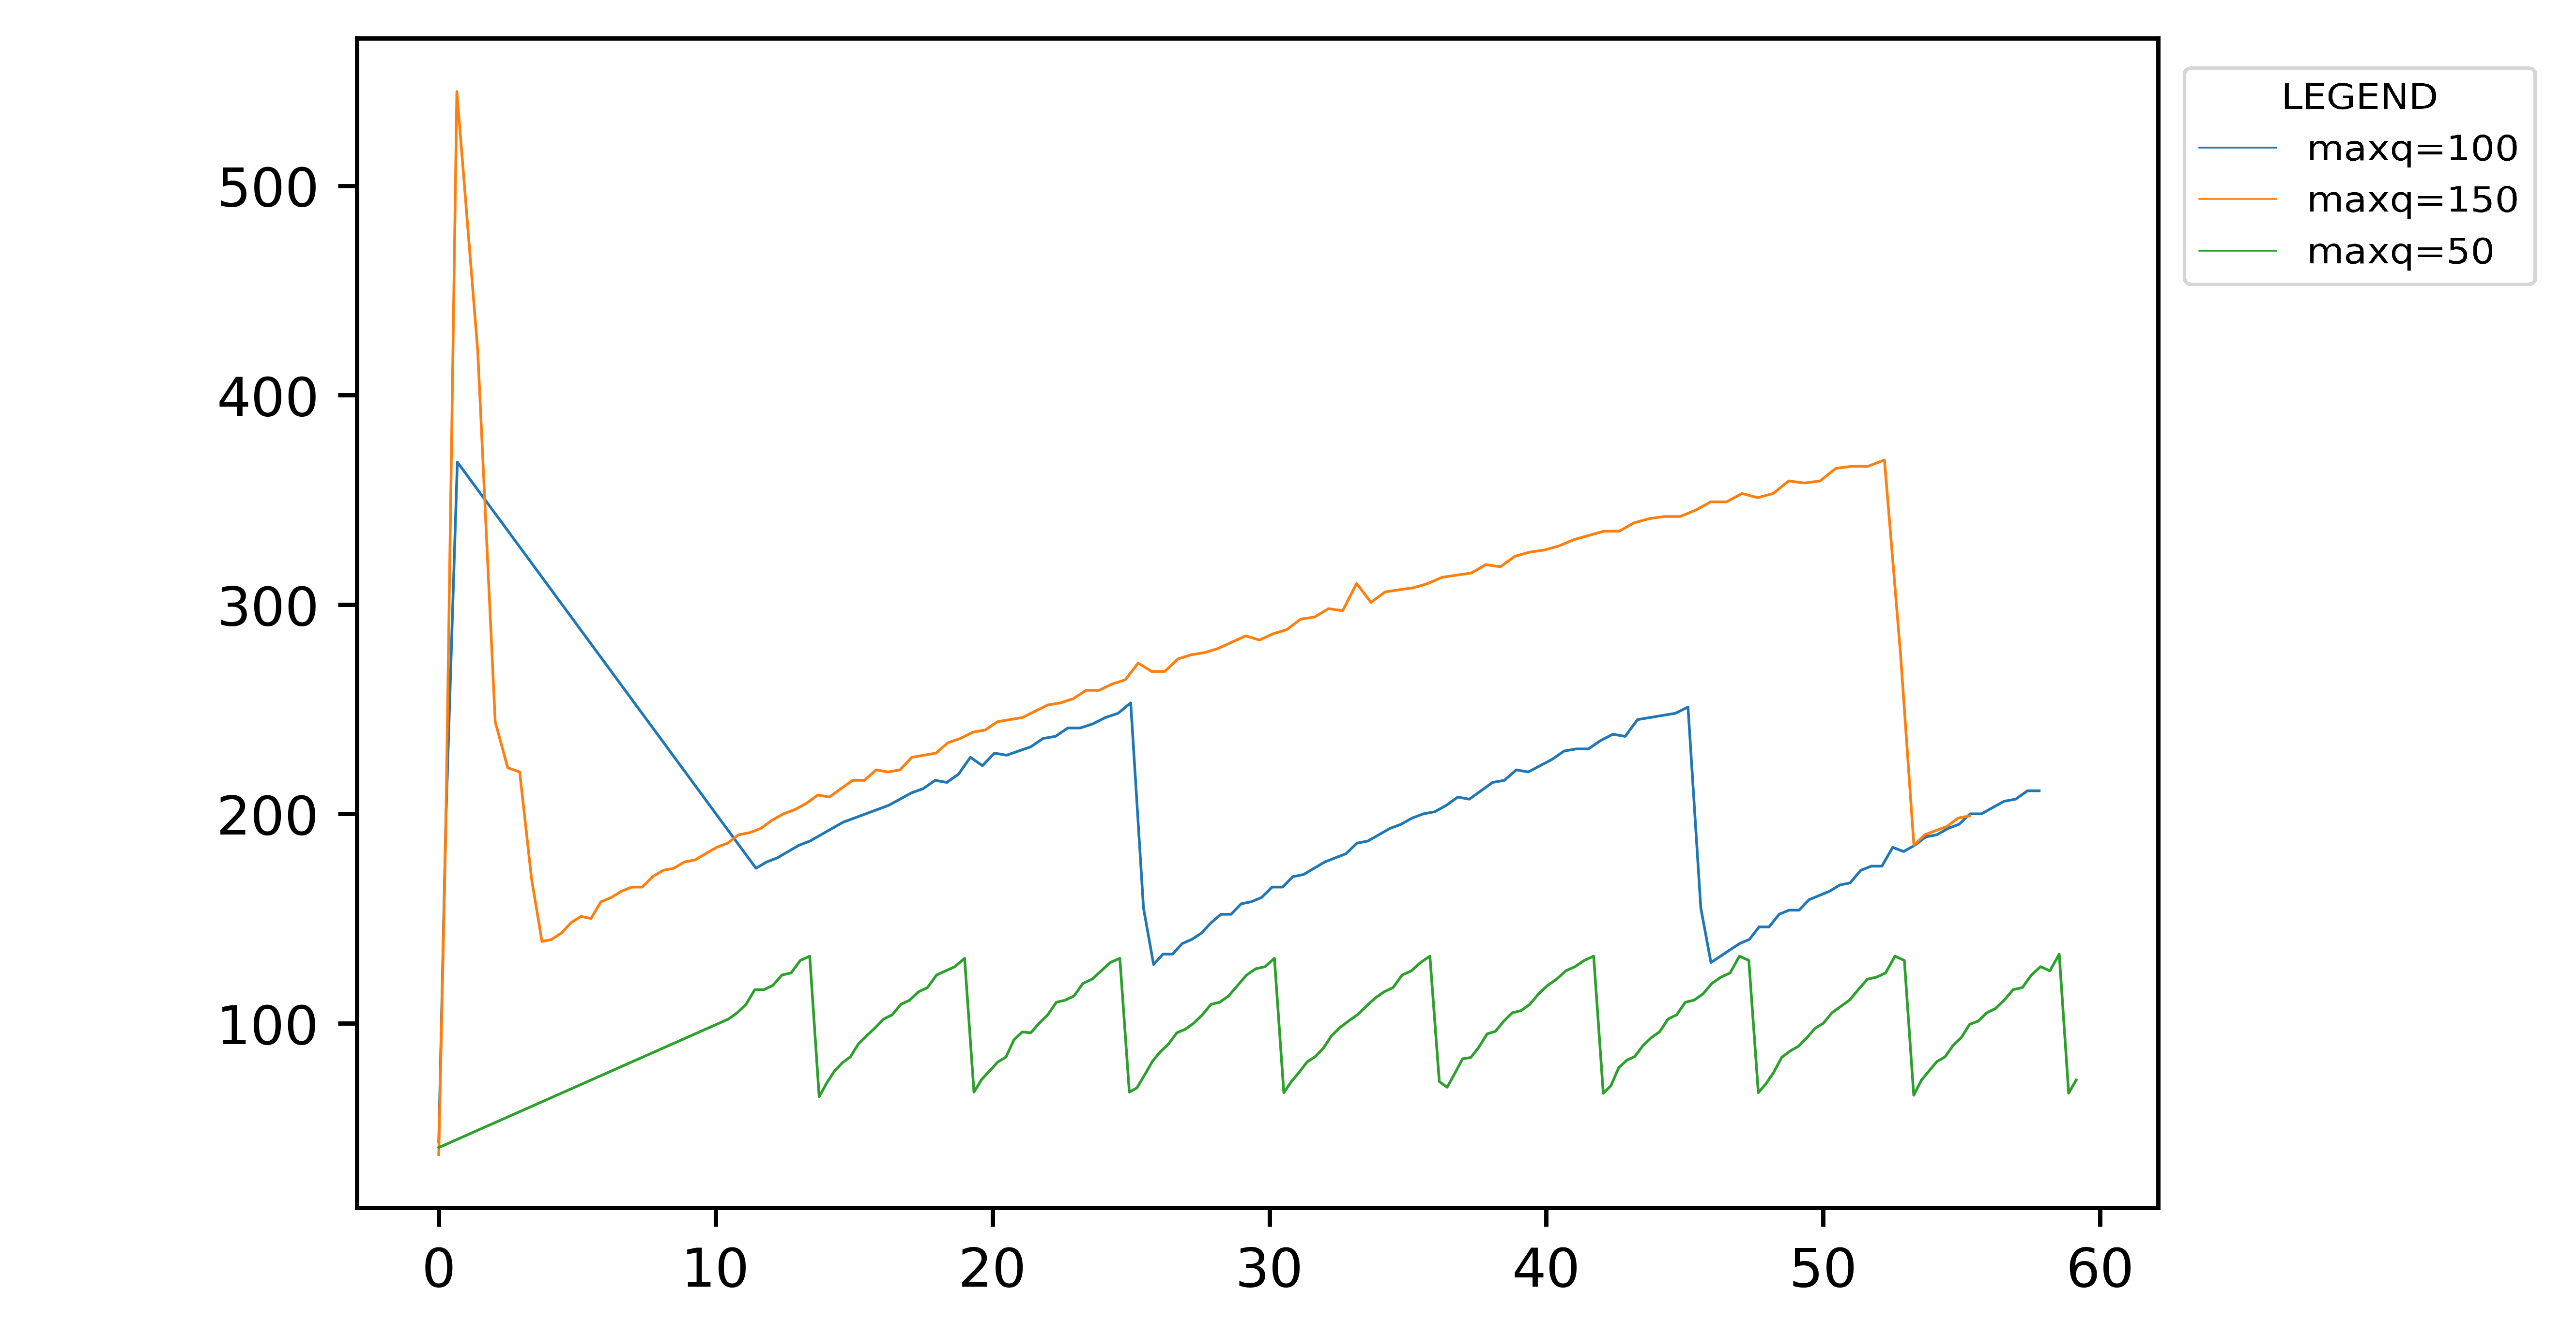
\includegraphics[width=280pt]{
            ../lab-07-pktq/readme.assets/rp-rtt.png}
        \caption{RTT 值 (单位: ms) 随时间 (单位: s) 变化曲线图} % 标题
    \end{figure}
\end{frame}
\begin{frame}{复现 bufferbloat}{实验 7: 数据包队列管理实验}
    \begin{figure}[h]
        \centering % 居中显示
        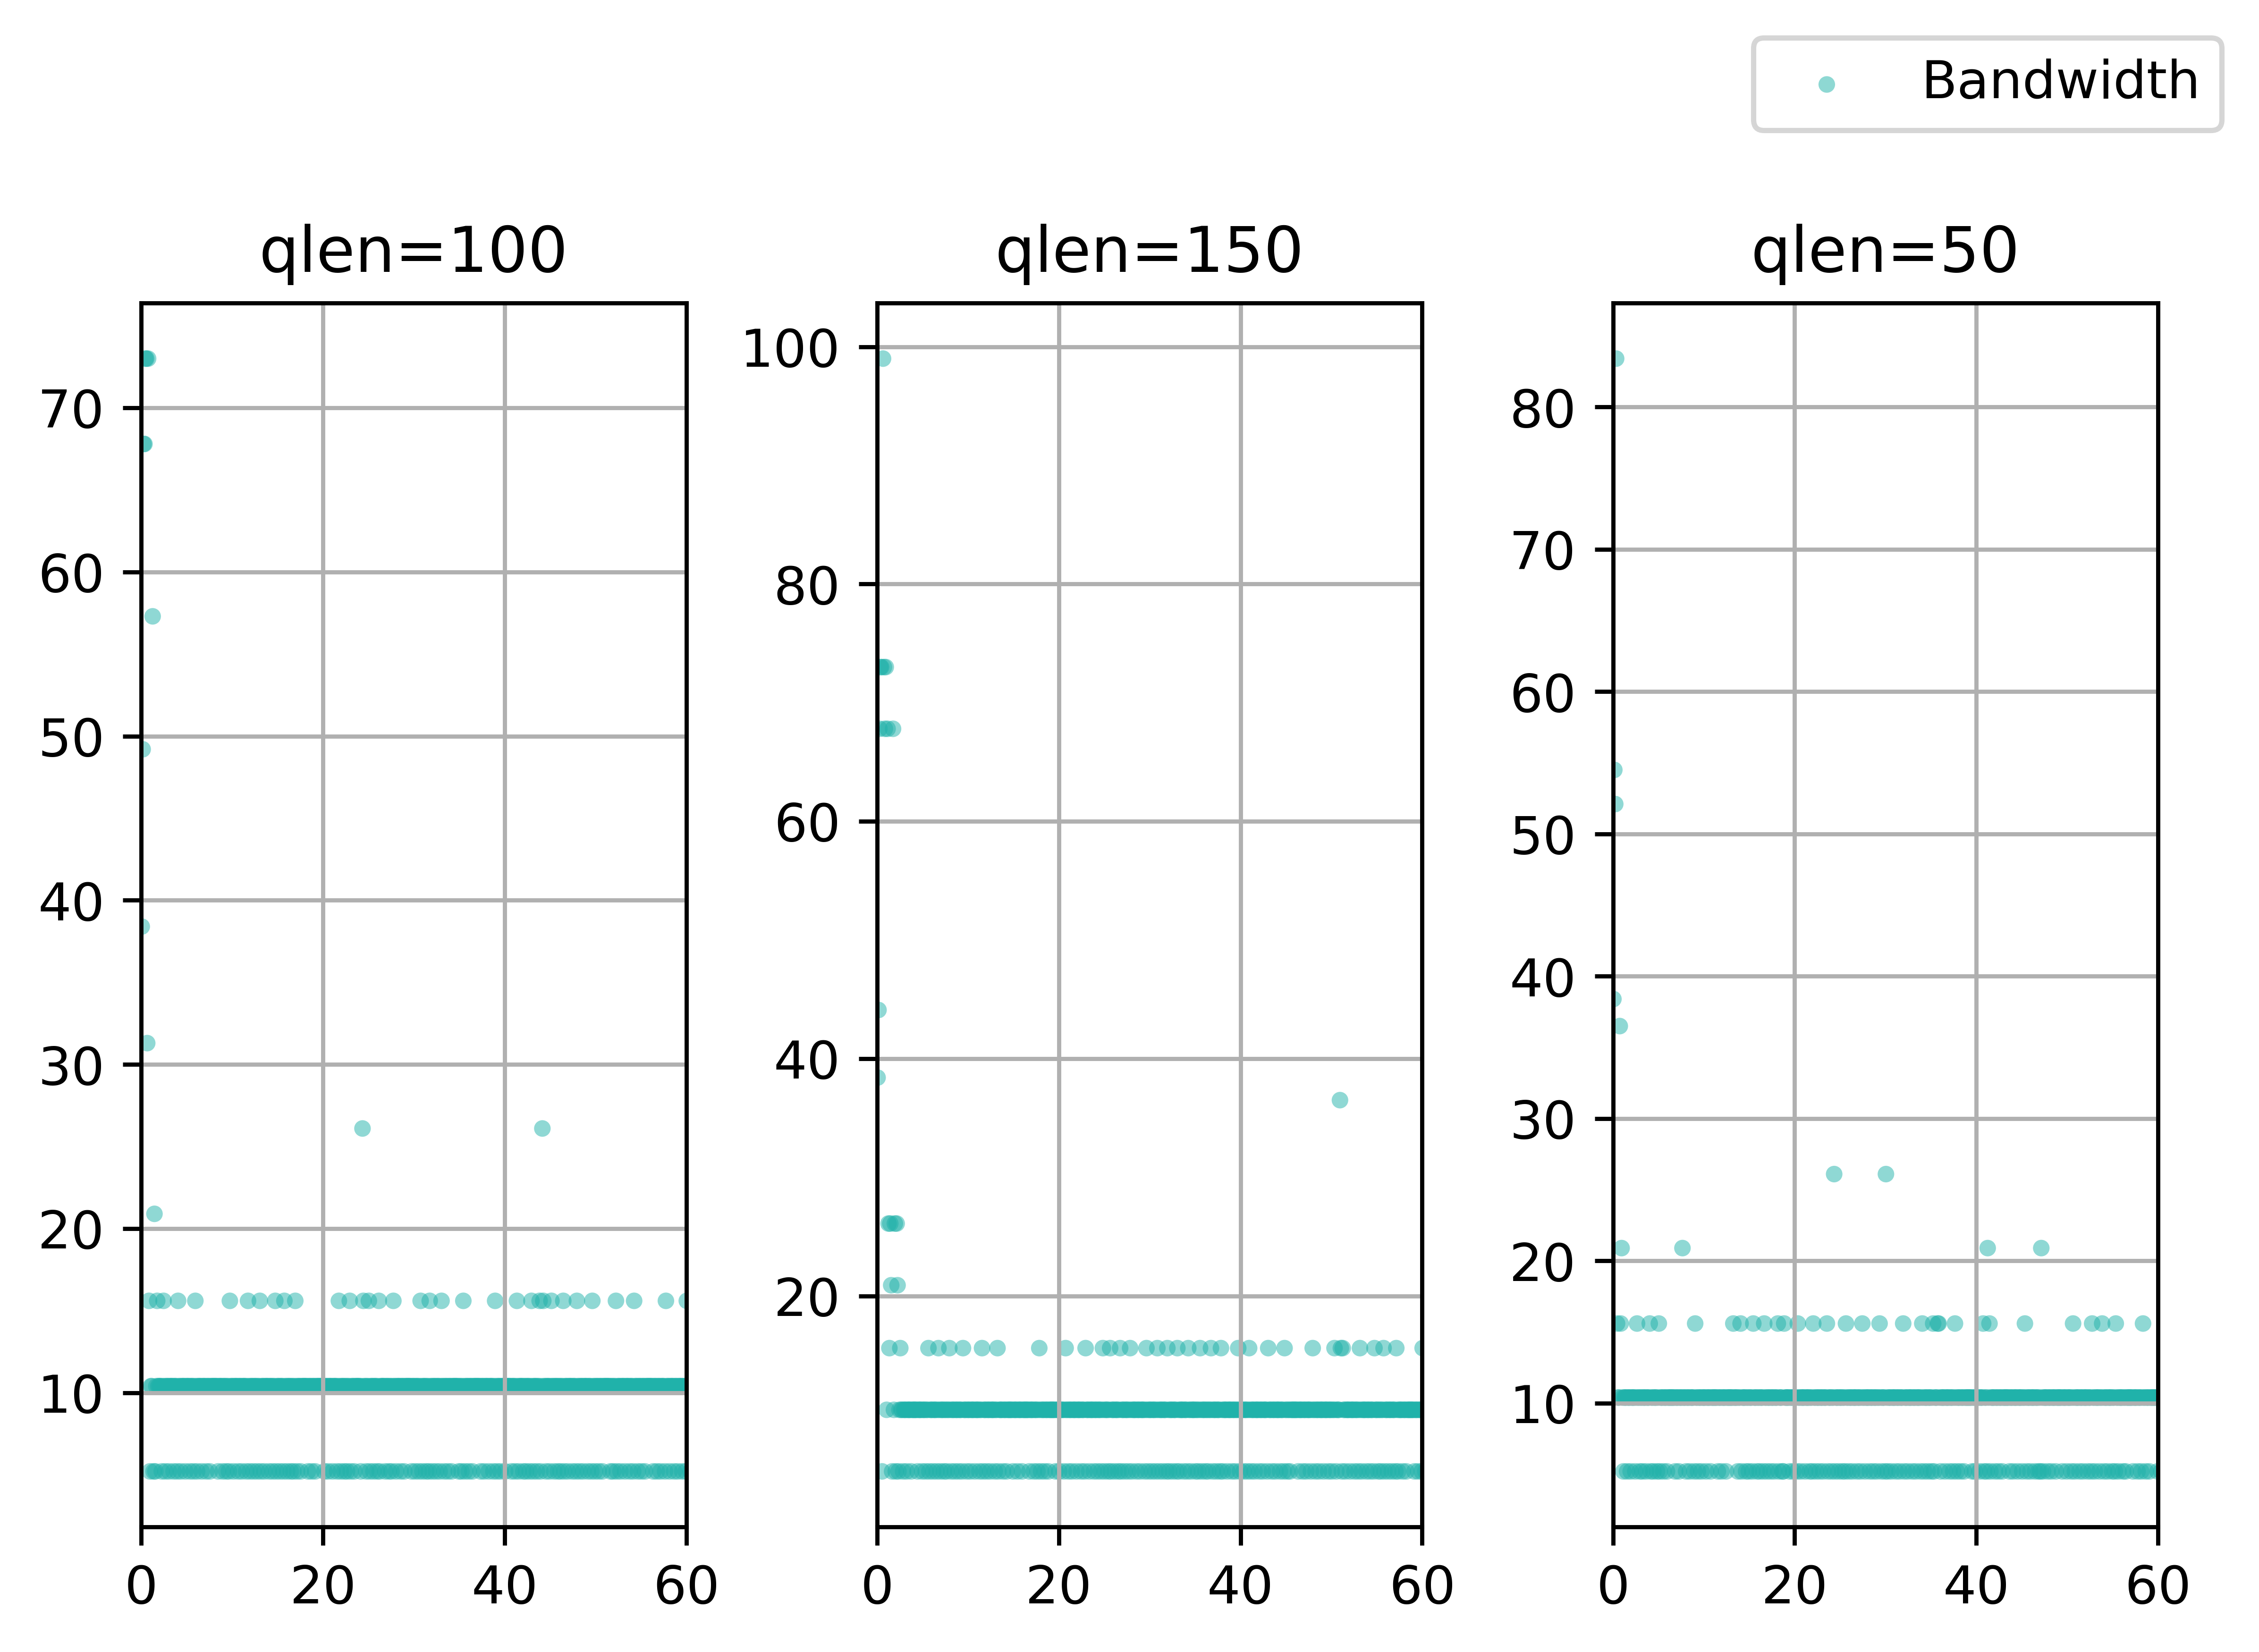
\includegraphics[width=180pt]{
            ../lab-07-pktq/readme.assets/rp-iperf-bw.png}
        \caption{iperf 测量中 Bandwidth 值
            (单位: Mbps) 随时间 (单位: s) 变化曲线图} % 标题
    \end{figure}
\end{frame}
\begin{frame}{复现 bufferbloat}{实验 7: 数据包队列管理实验}
    \begin{figure}[h]
        \centering % 居中显示
        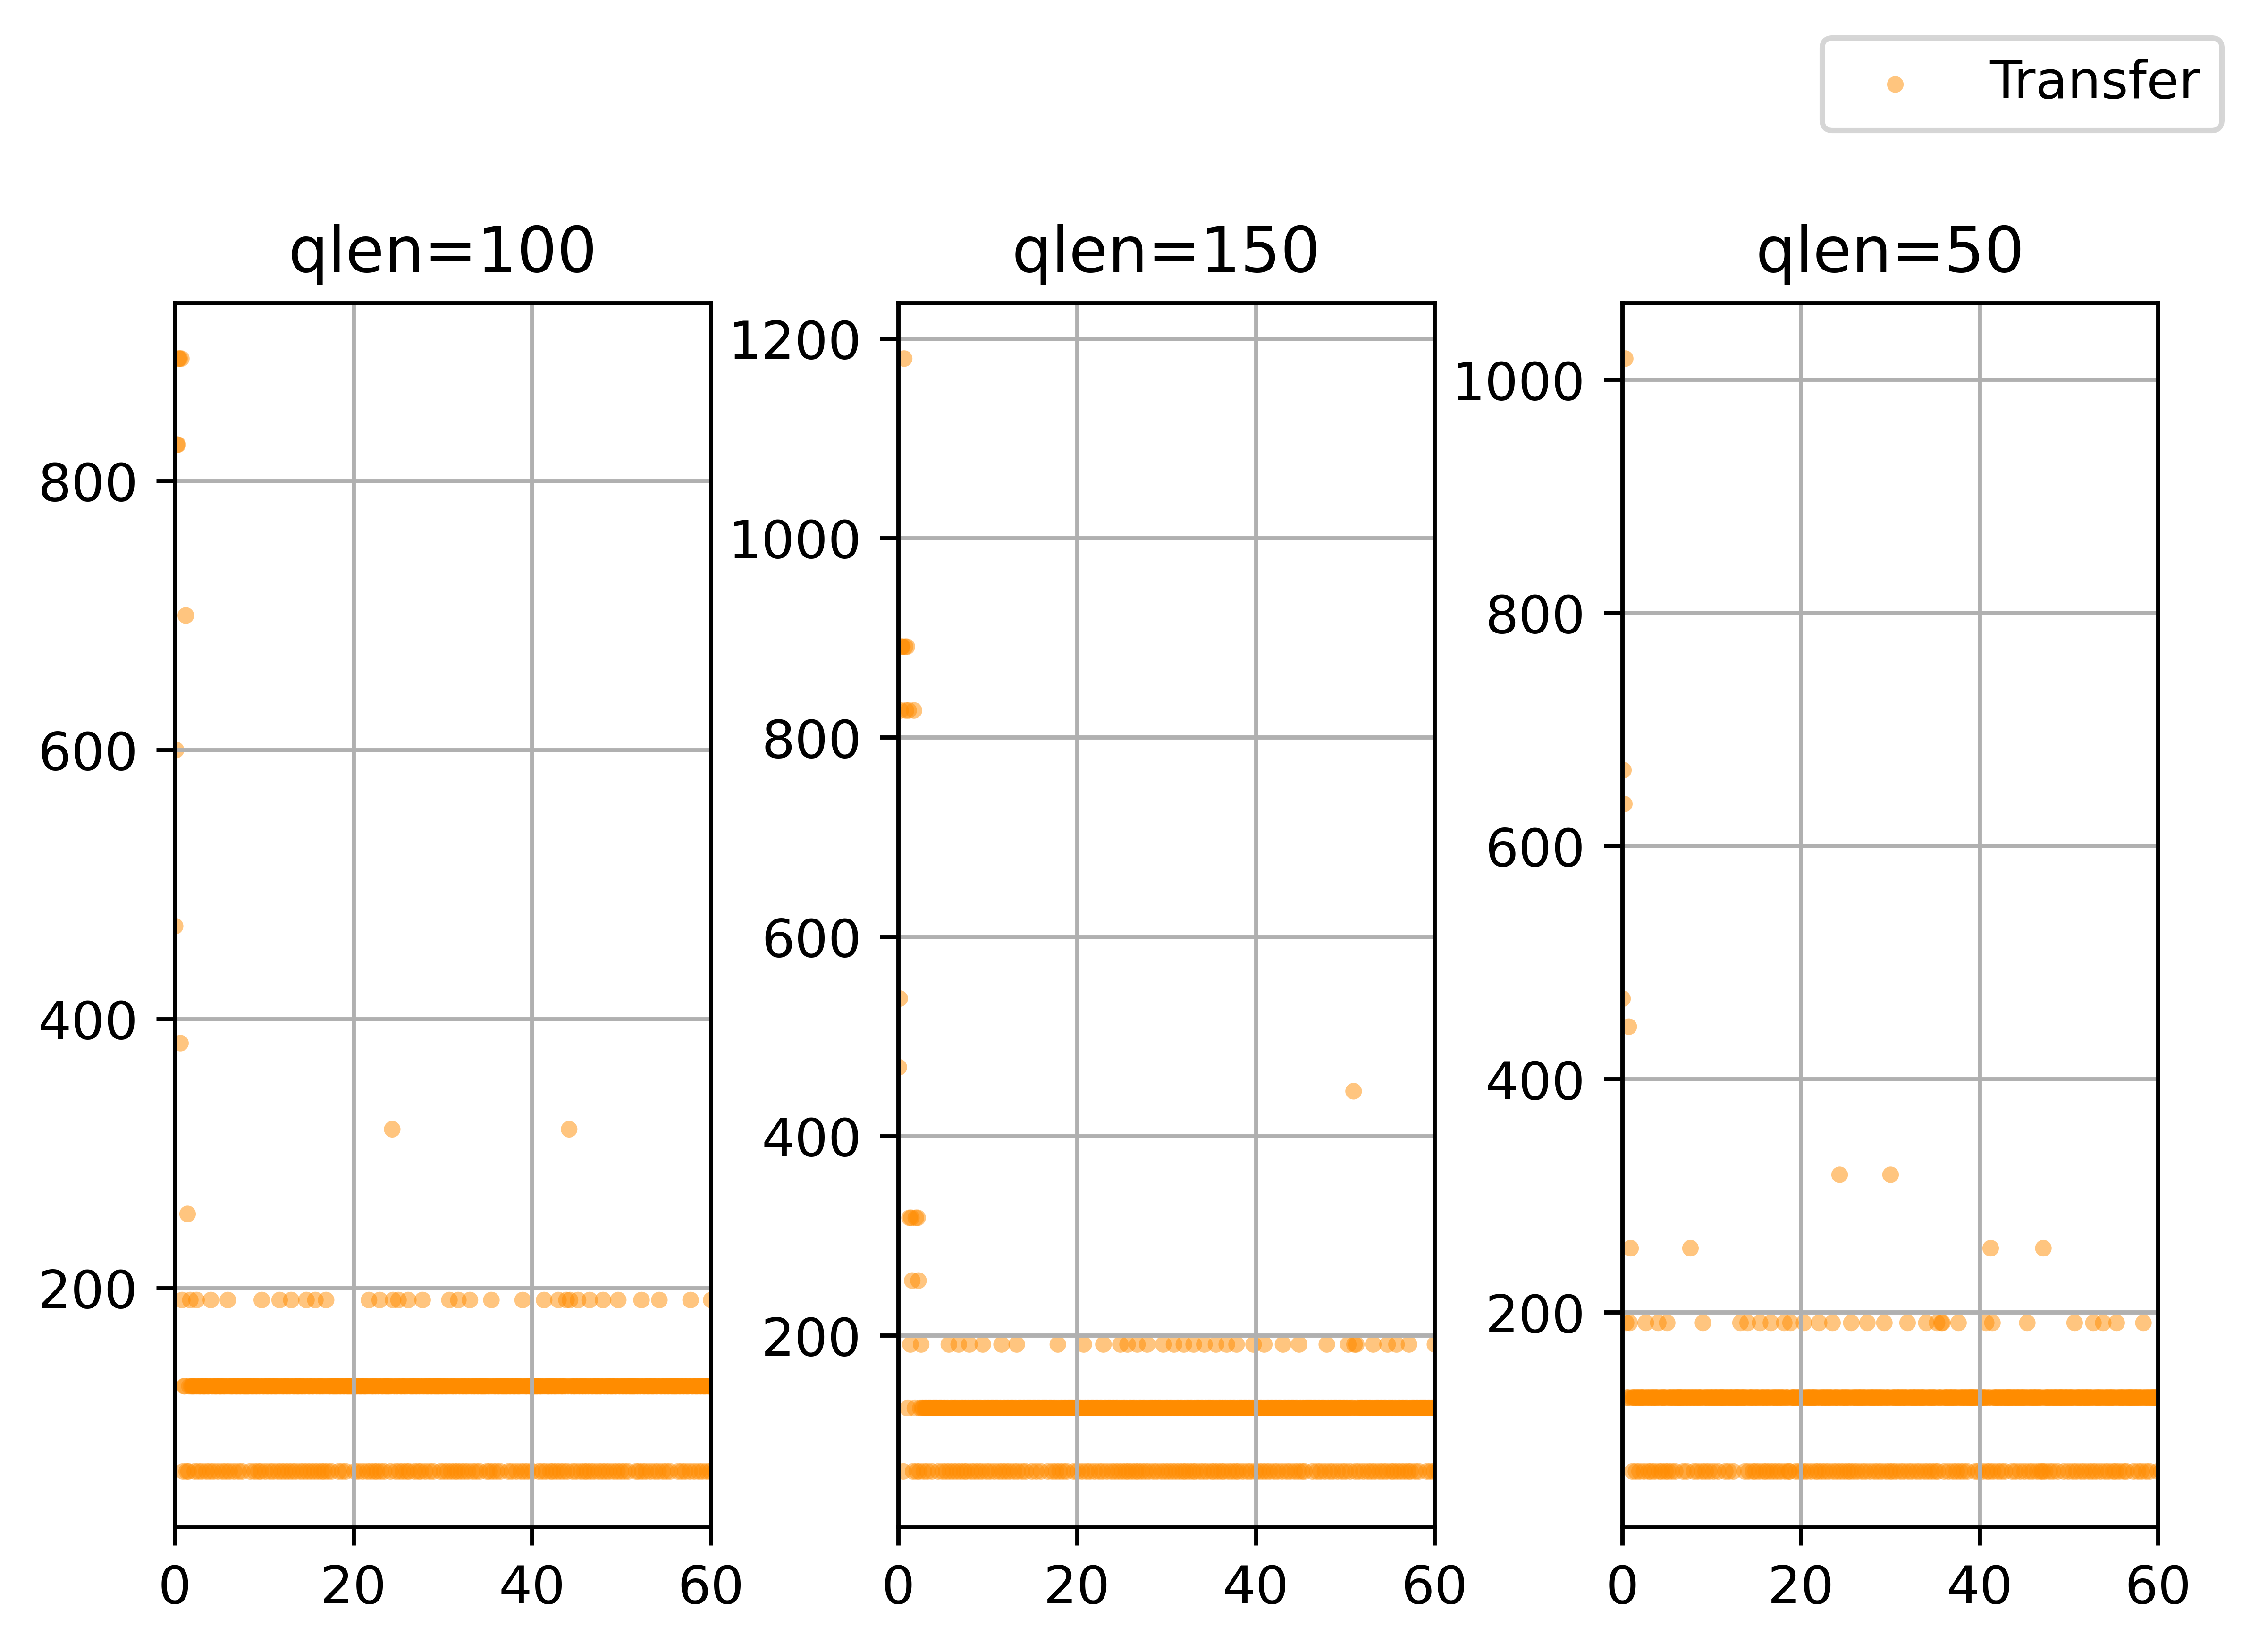
\includegraphics[width=180pt]{
            ../lab-07-pktq/readme.assets/rp-iperf-transfer.png}
        \caption{iperf 测量中 Transfer 值
            (单位: KB) 随时间 (单位: s) 变化曲线图} % 标题
    \end{figure}
\end{frame}

% 实验结果展示: 解决
\begin{frame}{复现 bufferbloat}{实验 7: 数据包队列管理实验}
    在动态带宽下, 使用不同算法解决bufferbloat问题, RTT值的变化:
    \begin{figure}[h]
        \centering % 居中显示
        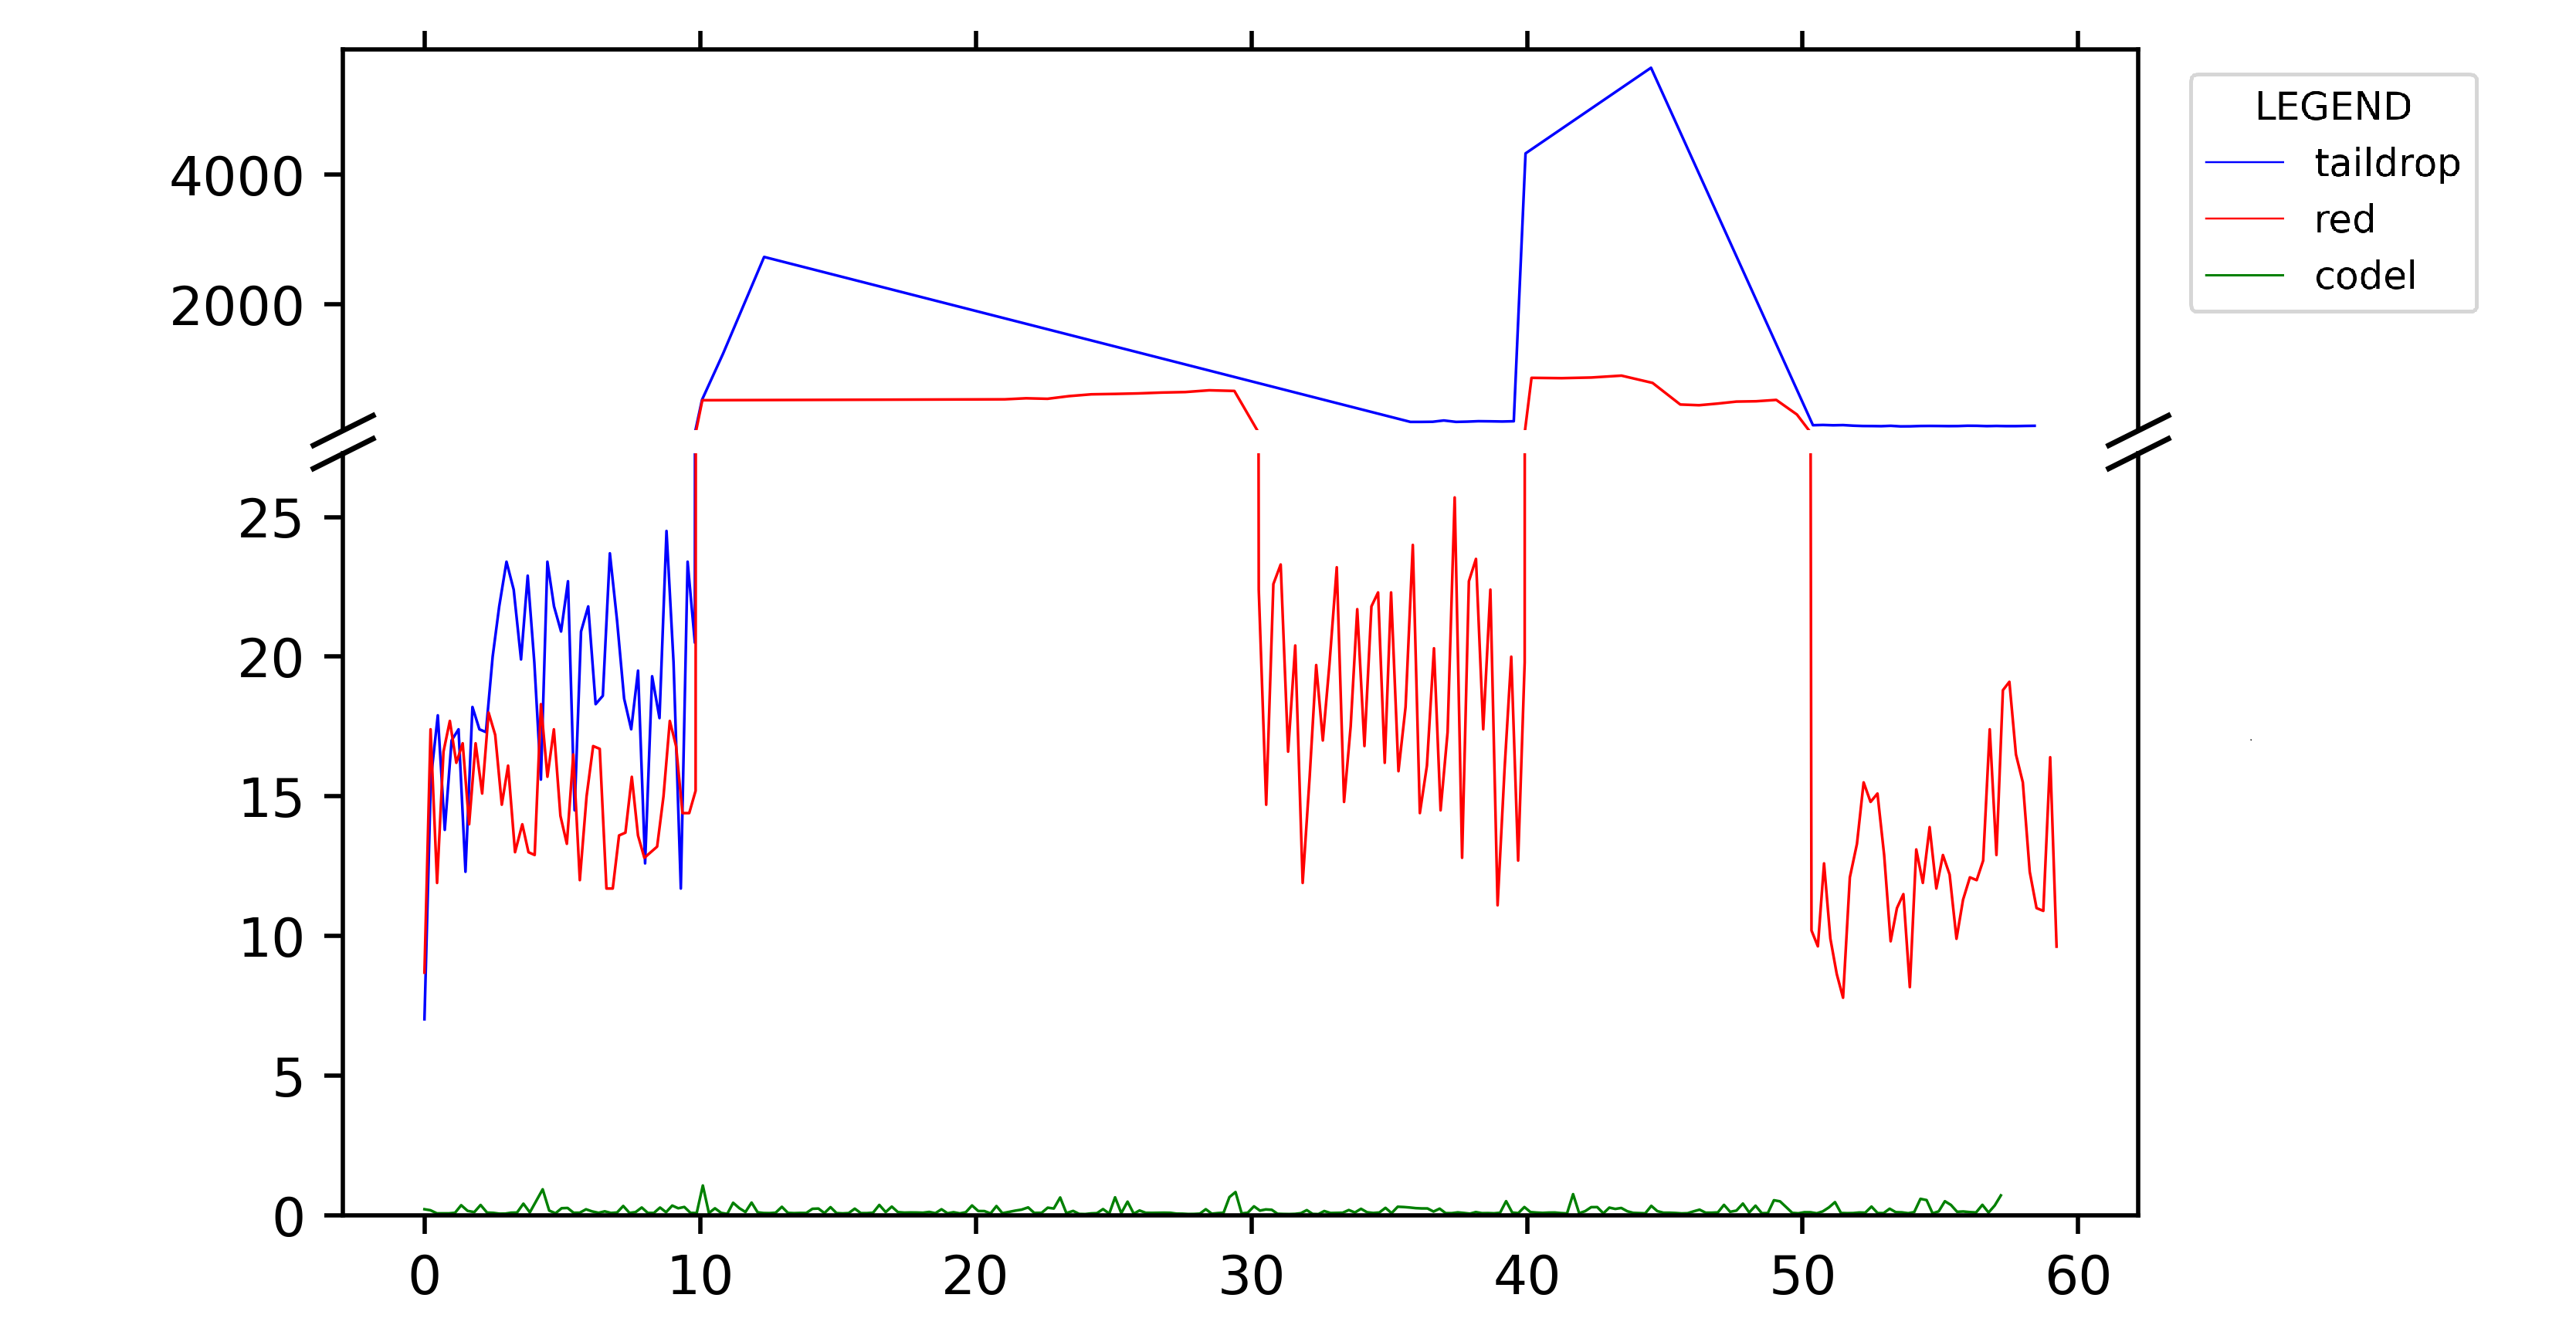
\includegraphics[width=280pt]{
            ../lab-07-pktq/readme.assets/mt-algos-rtt-fig.png}
        \caption{RTT 值 (单位: ms) 随时间 (单位: s) 变化曲线图} % 标题
    \end{figure}
\end{frame}

% 涉及的理论知识
\begin{frame}{涉及的理论知识}{实验 7: 数据包队列管理实验}
    \begin{figure}[h]
        \centering % 居中显示
        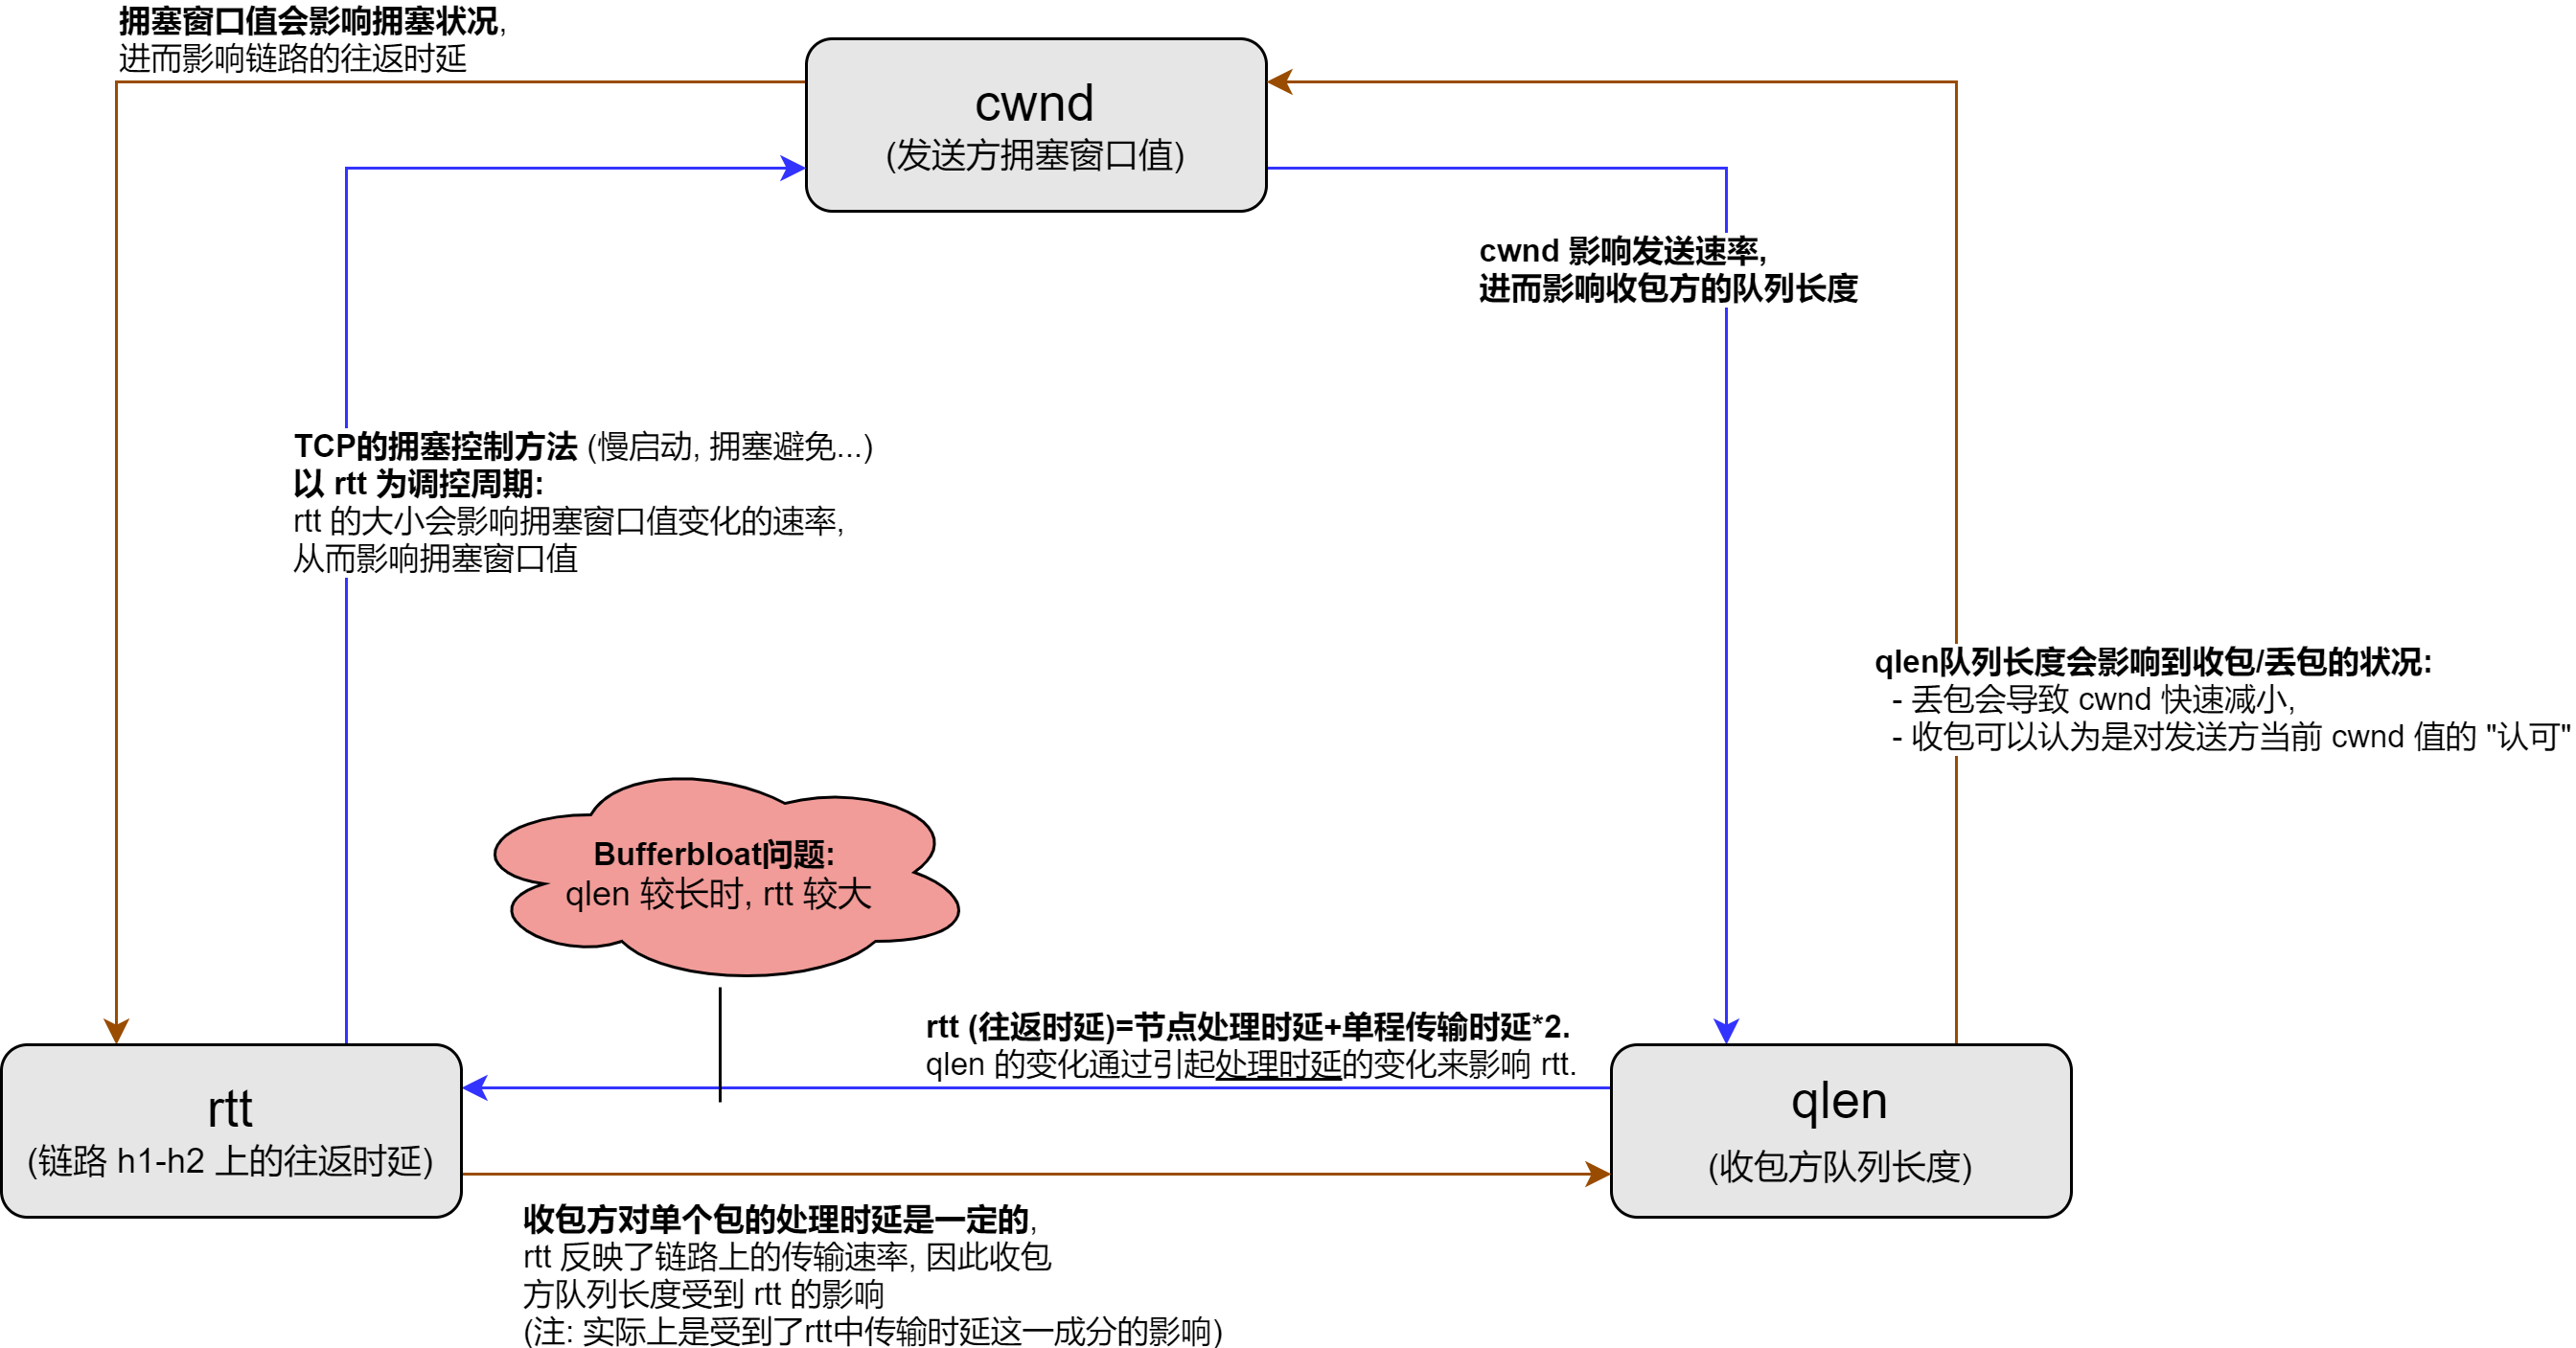
\includegraphics[width=340pt]{
            ../lab-07-pktq/readme.assets/lab-07-relation-between-cwnd-qlen-rtt.png}
        \caption{qlen, cwnd 和 rtt 的关系示意图} % 标题
    \end{figure}
\end{frame}

%%%%%%%%%%%%%%%%%%%%%%%%%%%%%%%%%%%%%%%%
%%%%%% 实验 9
\section{实验 9: 路由器转发实验}
% 节标题
\begin{frame}
    \sectionpage
\end{frame}

% 实验过程
\begin{frame}{实验过程}{实验 9: 路由器转发实验}
    \begin{block}{主要内容}
        1. 补充完成路由器程序, 在指定网络拓扑上运行,
        验证其功能;\\
        2. 构建符合要求的自定网络拓扑,
        测试路由器程序是否能正确完成其功能;
    \end{block}
    \begin{block}{需要补充的部分}
        1. 维护 ARP Cache, 支持增/查/老化;\\
        2. 借助 ARP Cache, 发送 ARP请求/回复, 处理 ARP 包;\\
        3. 封装 IP 层数据传输函数;\\
        4. 封装 ICMP 协议.
    \end{block}
\end{frame}

% 实验结果展示
\begin{frame}{实验结果展示: Ping test}{实验 9: 路由器转发实验}
    \begin{figure}[h]
        \centering % 居中显示
        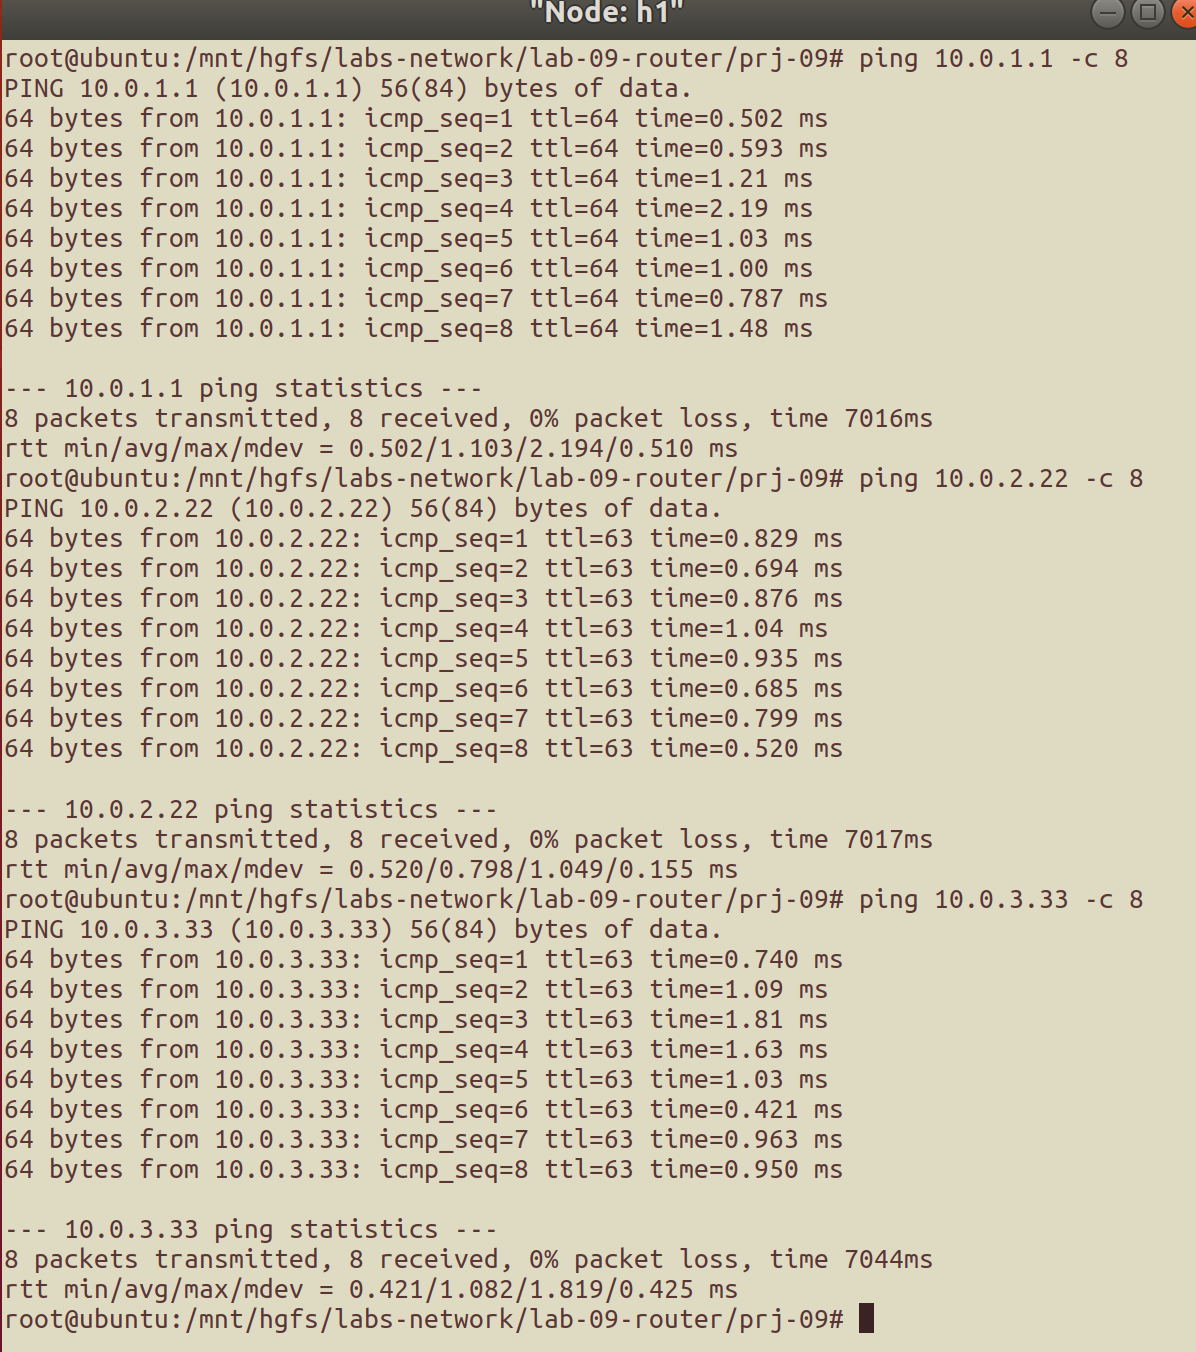
\includegraphics[width=150pt]{../lab-09-router/readme.assets/test-01-01.png}
        \caption{h1 ping r1, h2, h3} % 标题
    \end{figure}
\end{frame}
\begin{frame}{实验结果展示: Ping test}{实验 9: 路由器转发实验}
    \begin{figure}[h]
        \centering % 居中显示
        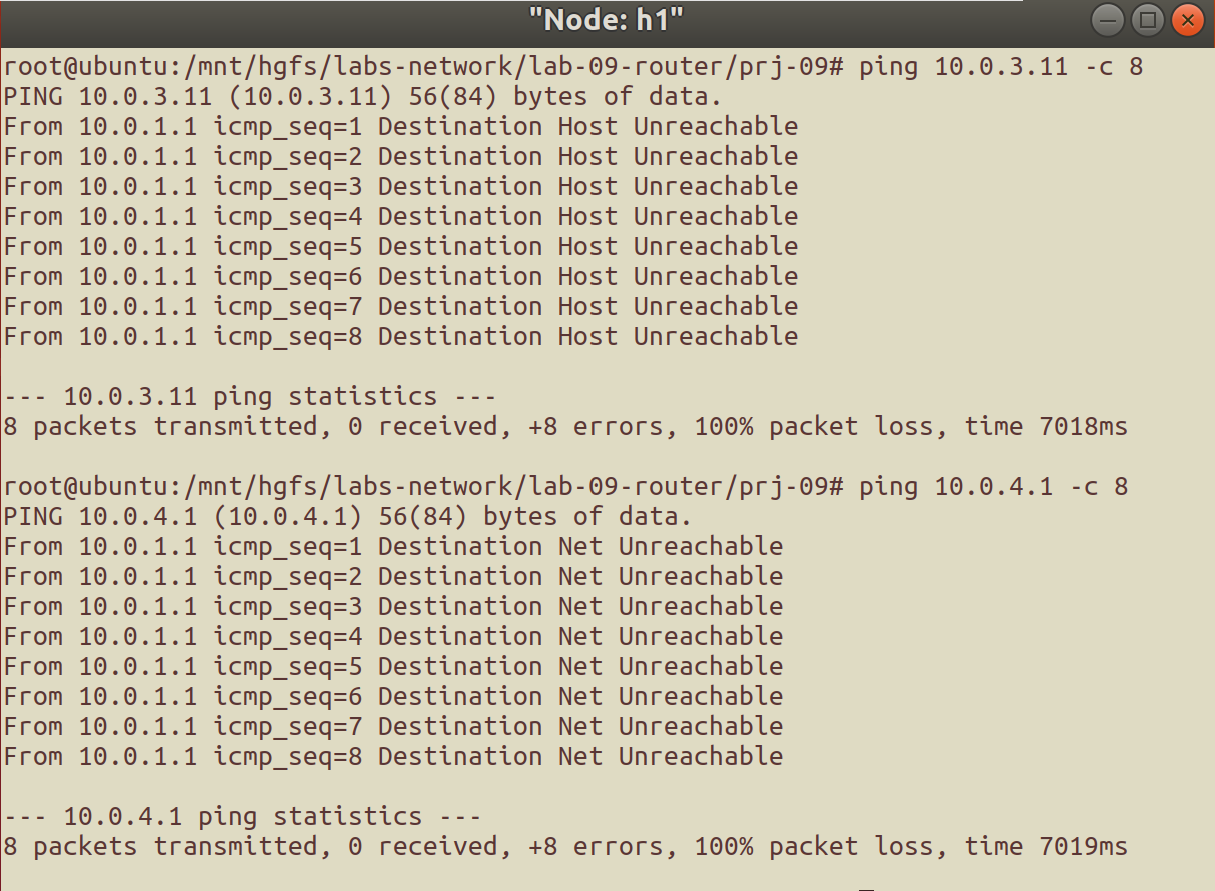
\includegraphics[width=200pt]{../lab-09-router/readme.assets/test-01-02.png}
        \caption{h1 ping 10.0.3.11, 10.0.4.1} % 标题
    \end{figure}
\end{frame}
\begin{frame}{实验结果展示: 在多路由器网络中测试}{实验 9: 路由器转发实验}
    \begin{figure}[h]
        \centering % 居中显示
        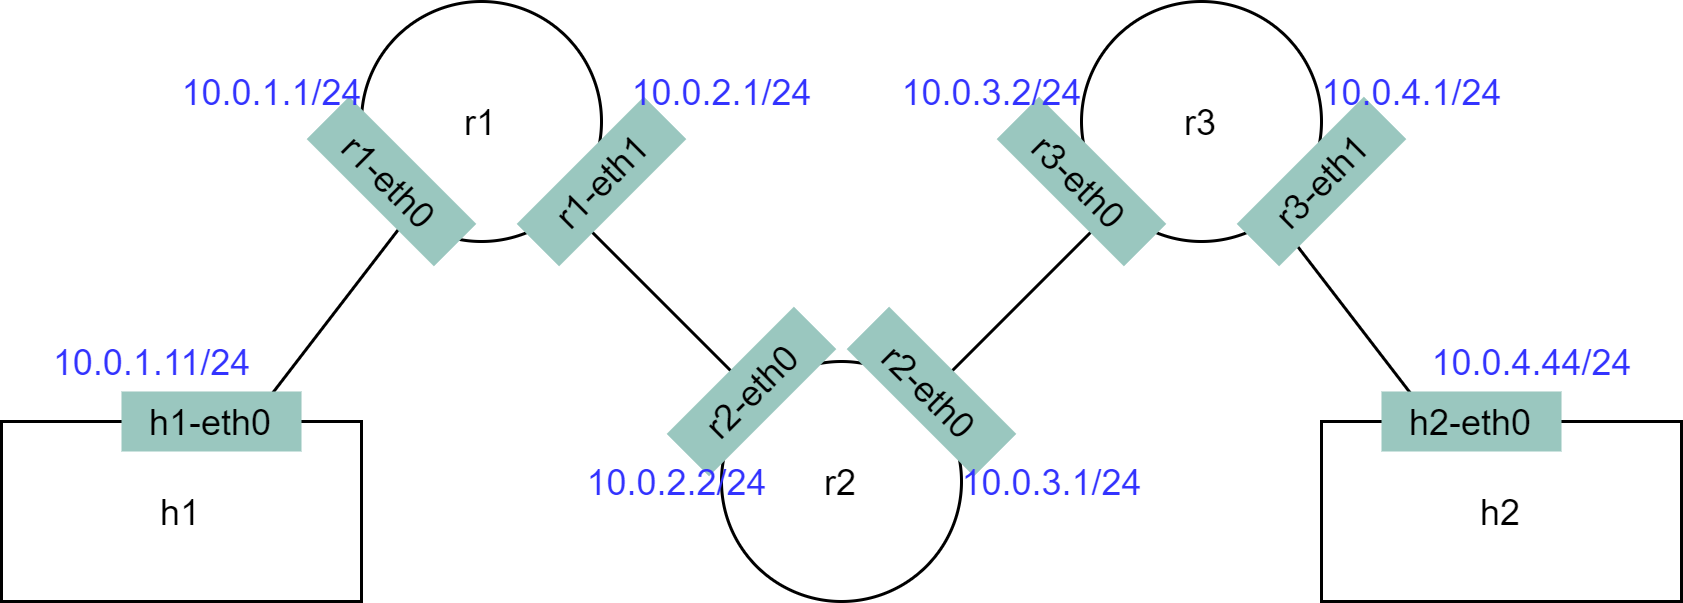
\includegraphics[width=230pt]{../lab-09-router/readme.assets/trace-path.png}
        \caption{构造拓扑} % 标题
    \end{figure}
\end{frame}
\begin{frame}{实验结果展示: 在多路由器网络中测试}{实验 9: 路由器转发实验}
    \begin{figure}[h]
        \centering % 居中显示
        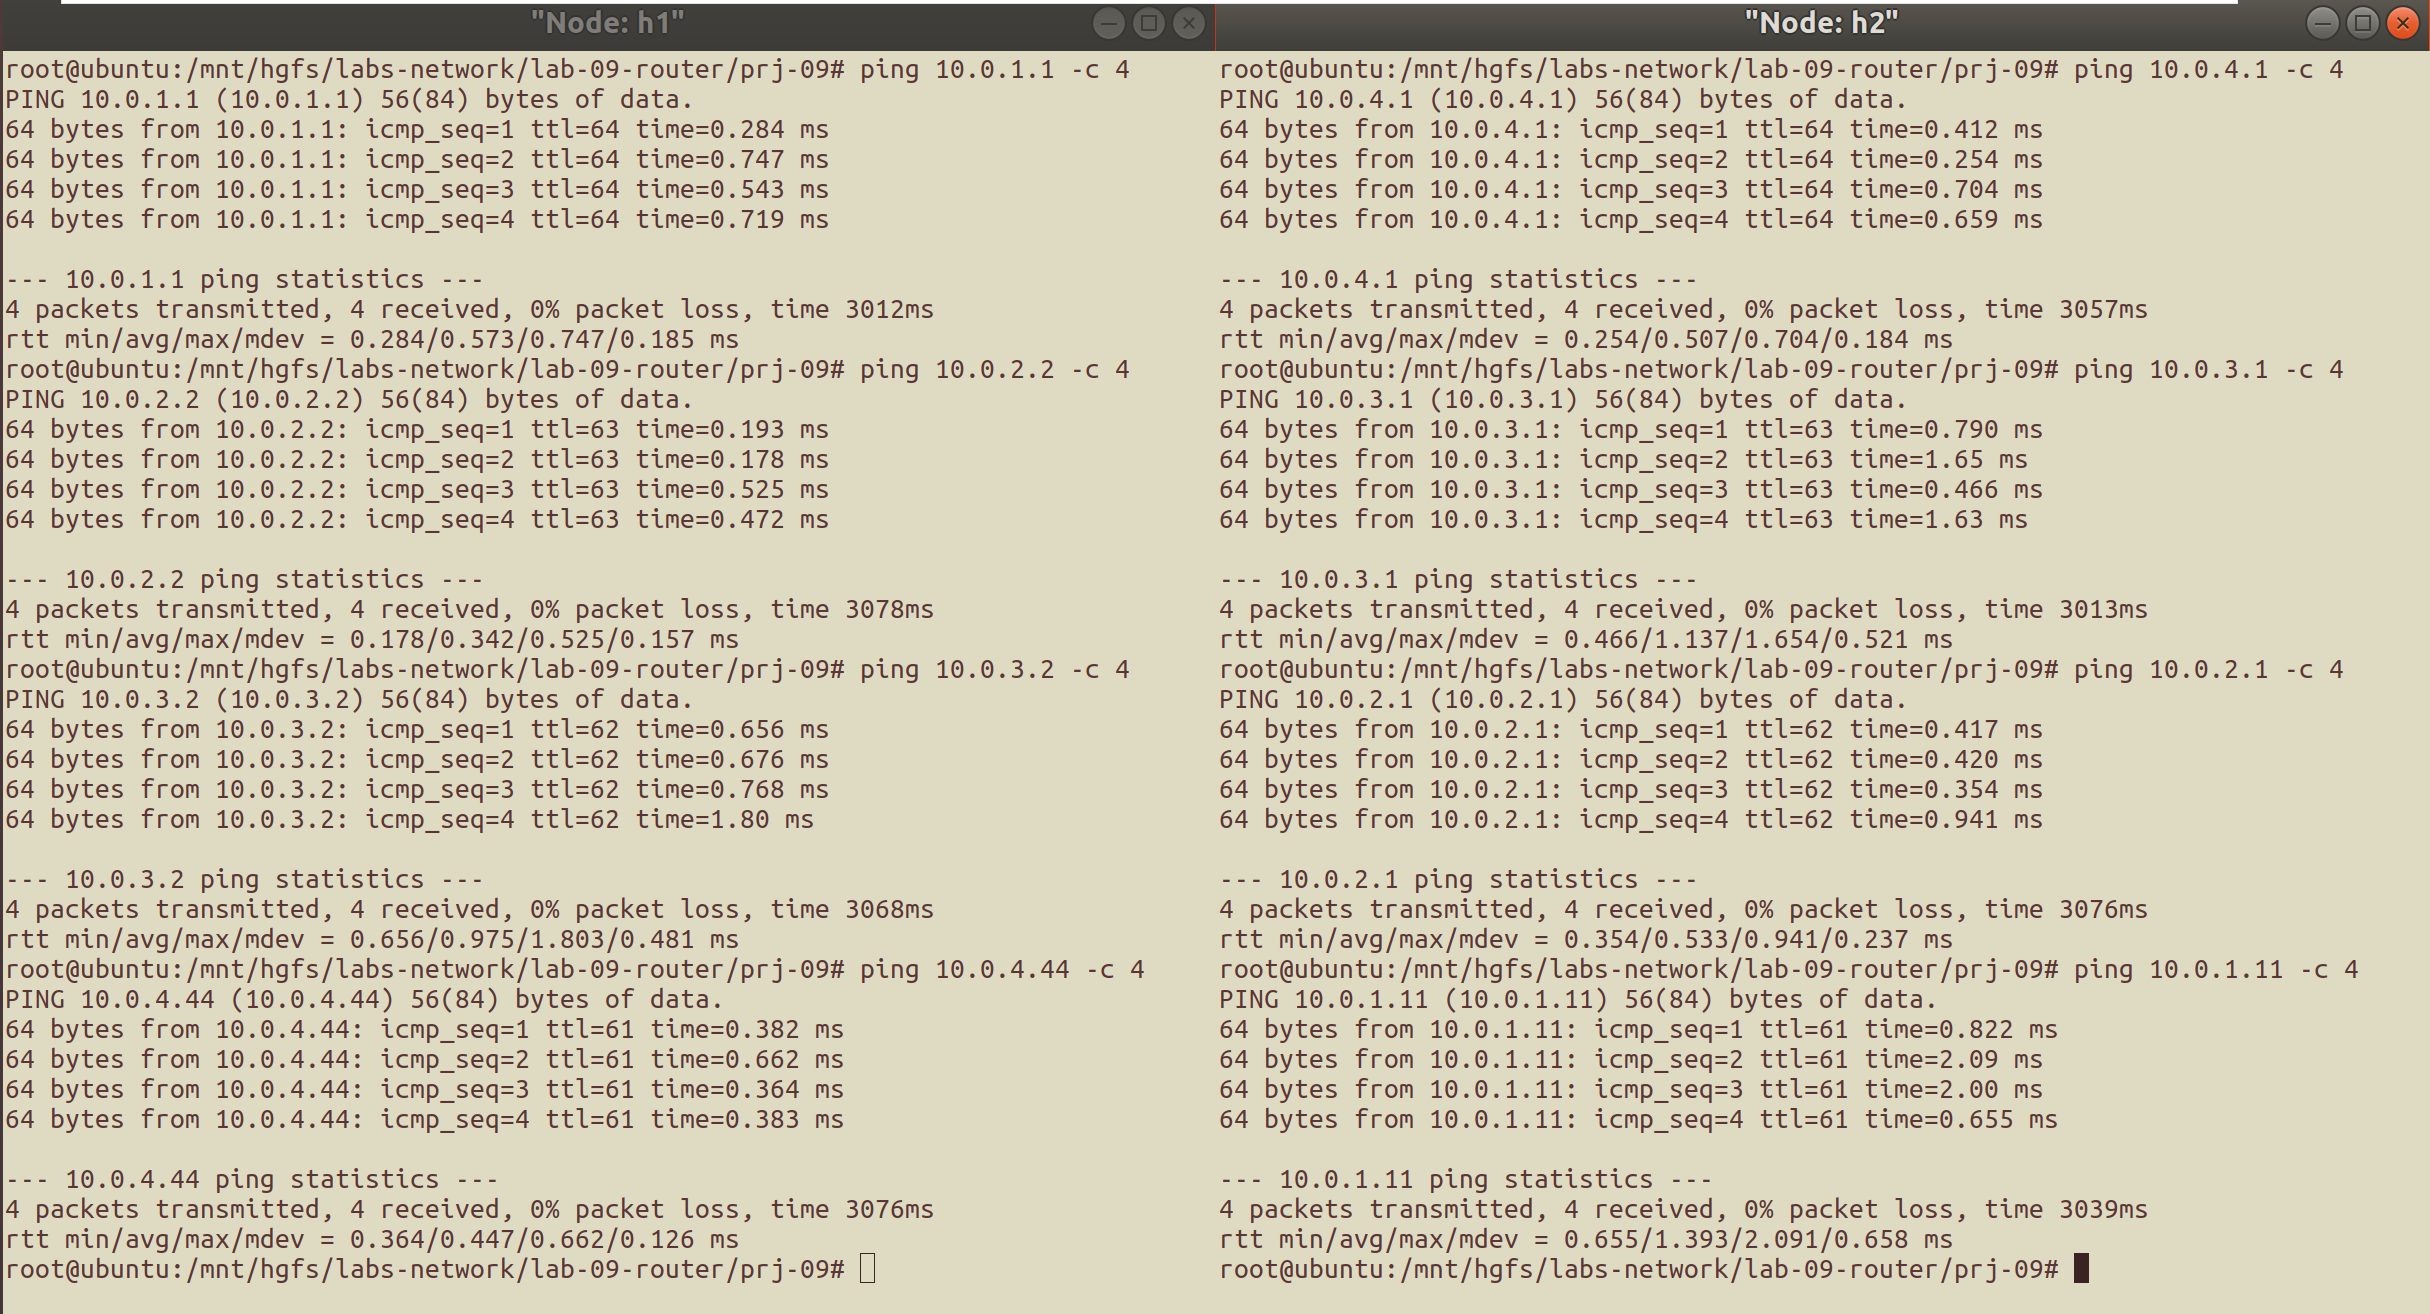
\includegraphics[width=270pt]{../lab-09-router/readme.assets/trace-connectivity.png}
        \caption{连通性测试} % 标题
    \end{figure}
\end{frame}
\begin{frame}{实验结果展示: 在多路由器网络中测试}{实验 9: 路由器转发实验}
    \begin{figure}[h]
        \centering % 居中显示
        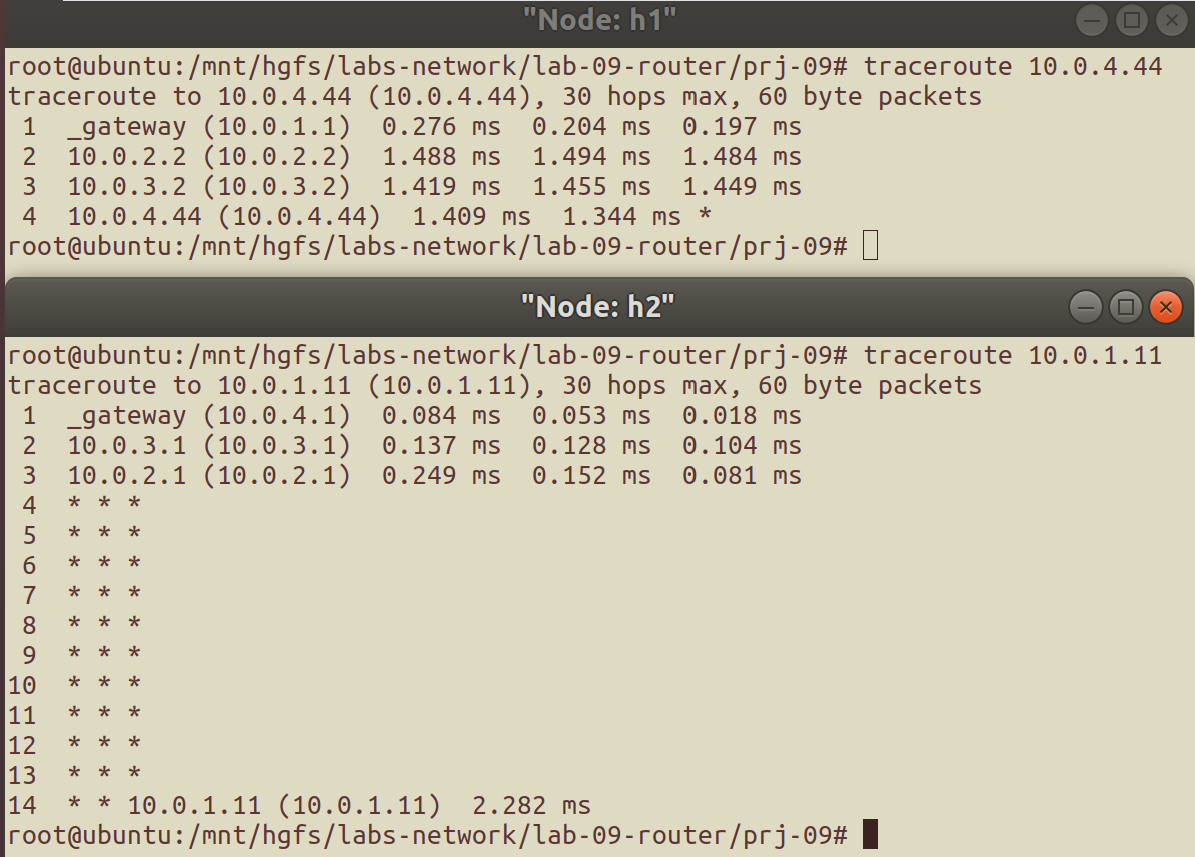
\includegraphics[width=250pt]{../lab-09-router/readme.assets/trace-route-res.png}
        \caption{路径测试} % 标题
    \end{figure}
\end{frame}

% 实验反思
\begin{frame}{实验反思}{实验 9: 路由器转发实验}
    \begin{alertblock}{调试中出现的问题}
        1. 源地址/目的地址和网关混淆;\\
        2. 应该使用网络字节序的地方忘记转换;\\
        3. 忽视了路由器节点的能力限制,
        在应该丢弃数据包的时候胡乱发包;\\
        4. 与框架的适配没做好, 出现 double free 的情况;\\
        5. 数据包的封装未严格按照协议格式,
        封装过程中字节序出错
        (本次实验中出现过拷贝错误和字节序混乱的问题);\\
        6. 变量类型混淆, 比如 'u32' 和 'int'
        一个是有符号一个是无符号, 最好不要将它们混在一起比较,
        若需比较最好使用同一数据类型;\\
        7. 单个 'mutex' 的互斥使用区分不清楚, 造成死锁.
    \end{alertblock}
\end{frame}
\begin{frame}{程序的性能限制}{实验 9: 路由器转发实验}
    \begin{alertblock}{问题产生现象}
        在进行对主机不可达情形进行测试时, 发现偶尔会有丢包的情况发生.
    \end{alertblock}
    \begin{block}{排查原因}
        按第一部分测试, 执行 'ping 10.0.3.11 -c 4' ,
        并在 h1 节点上使用 wireshark 进行抓包,
        发现 r1 发送了4个ICMP端口不可达消息,
        而 h1 只收到了一个. (图见下页)
    \end{block}
\end{frame}
\begin{frame}{程序的性能限制}{实验 9: 路由器转发实验}
    \begin{block}{排查原因}
        \begin{figure}[h]
            \centering % 居中显示
            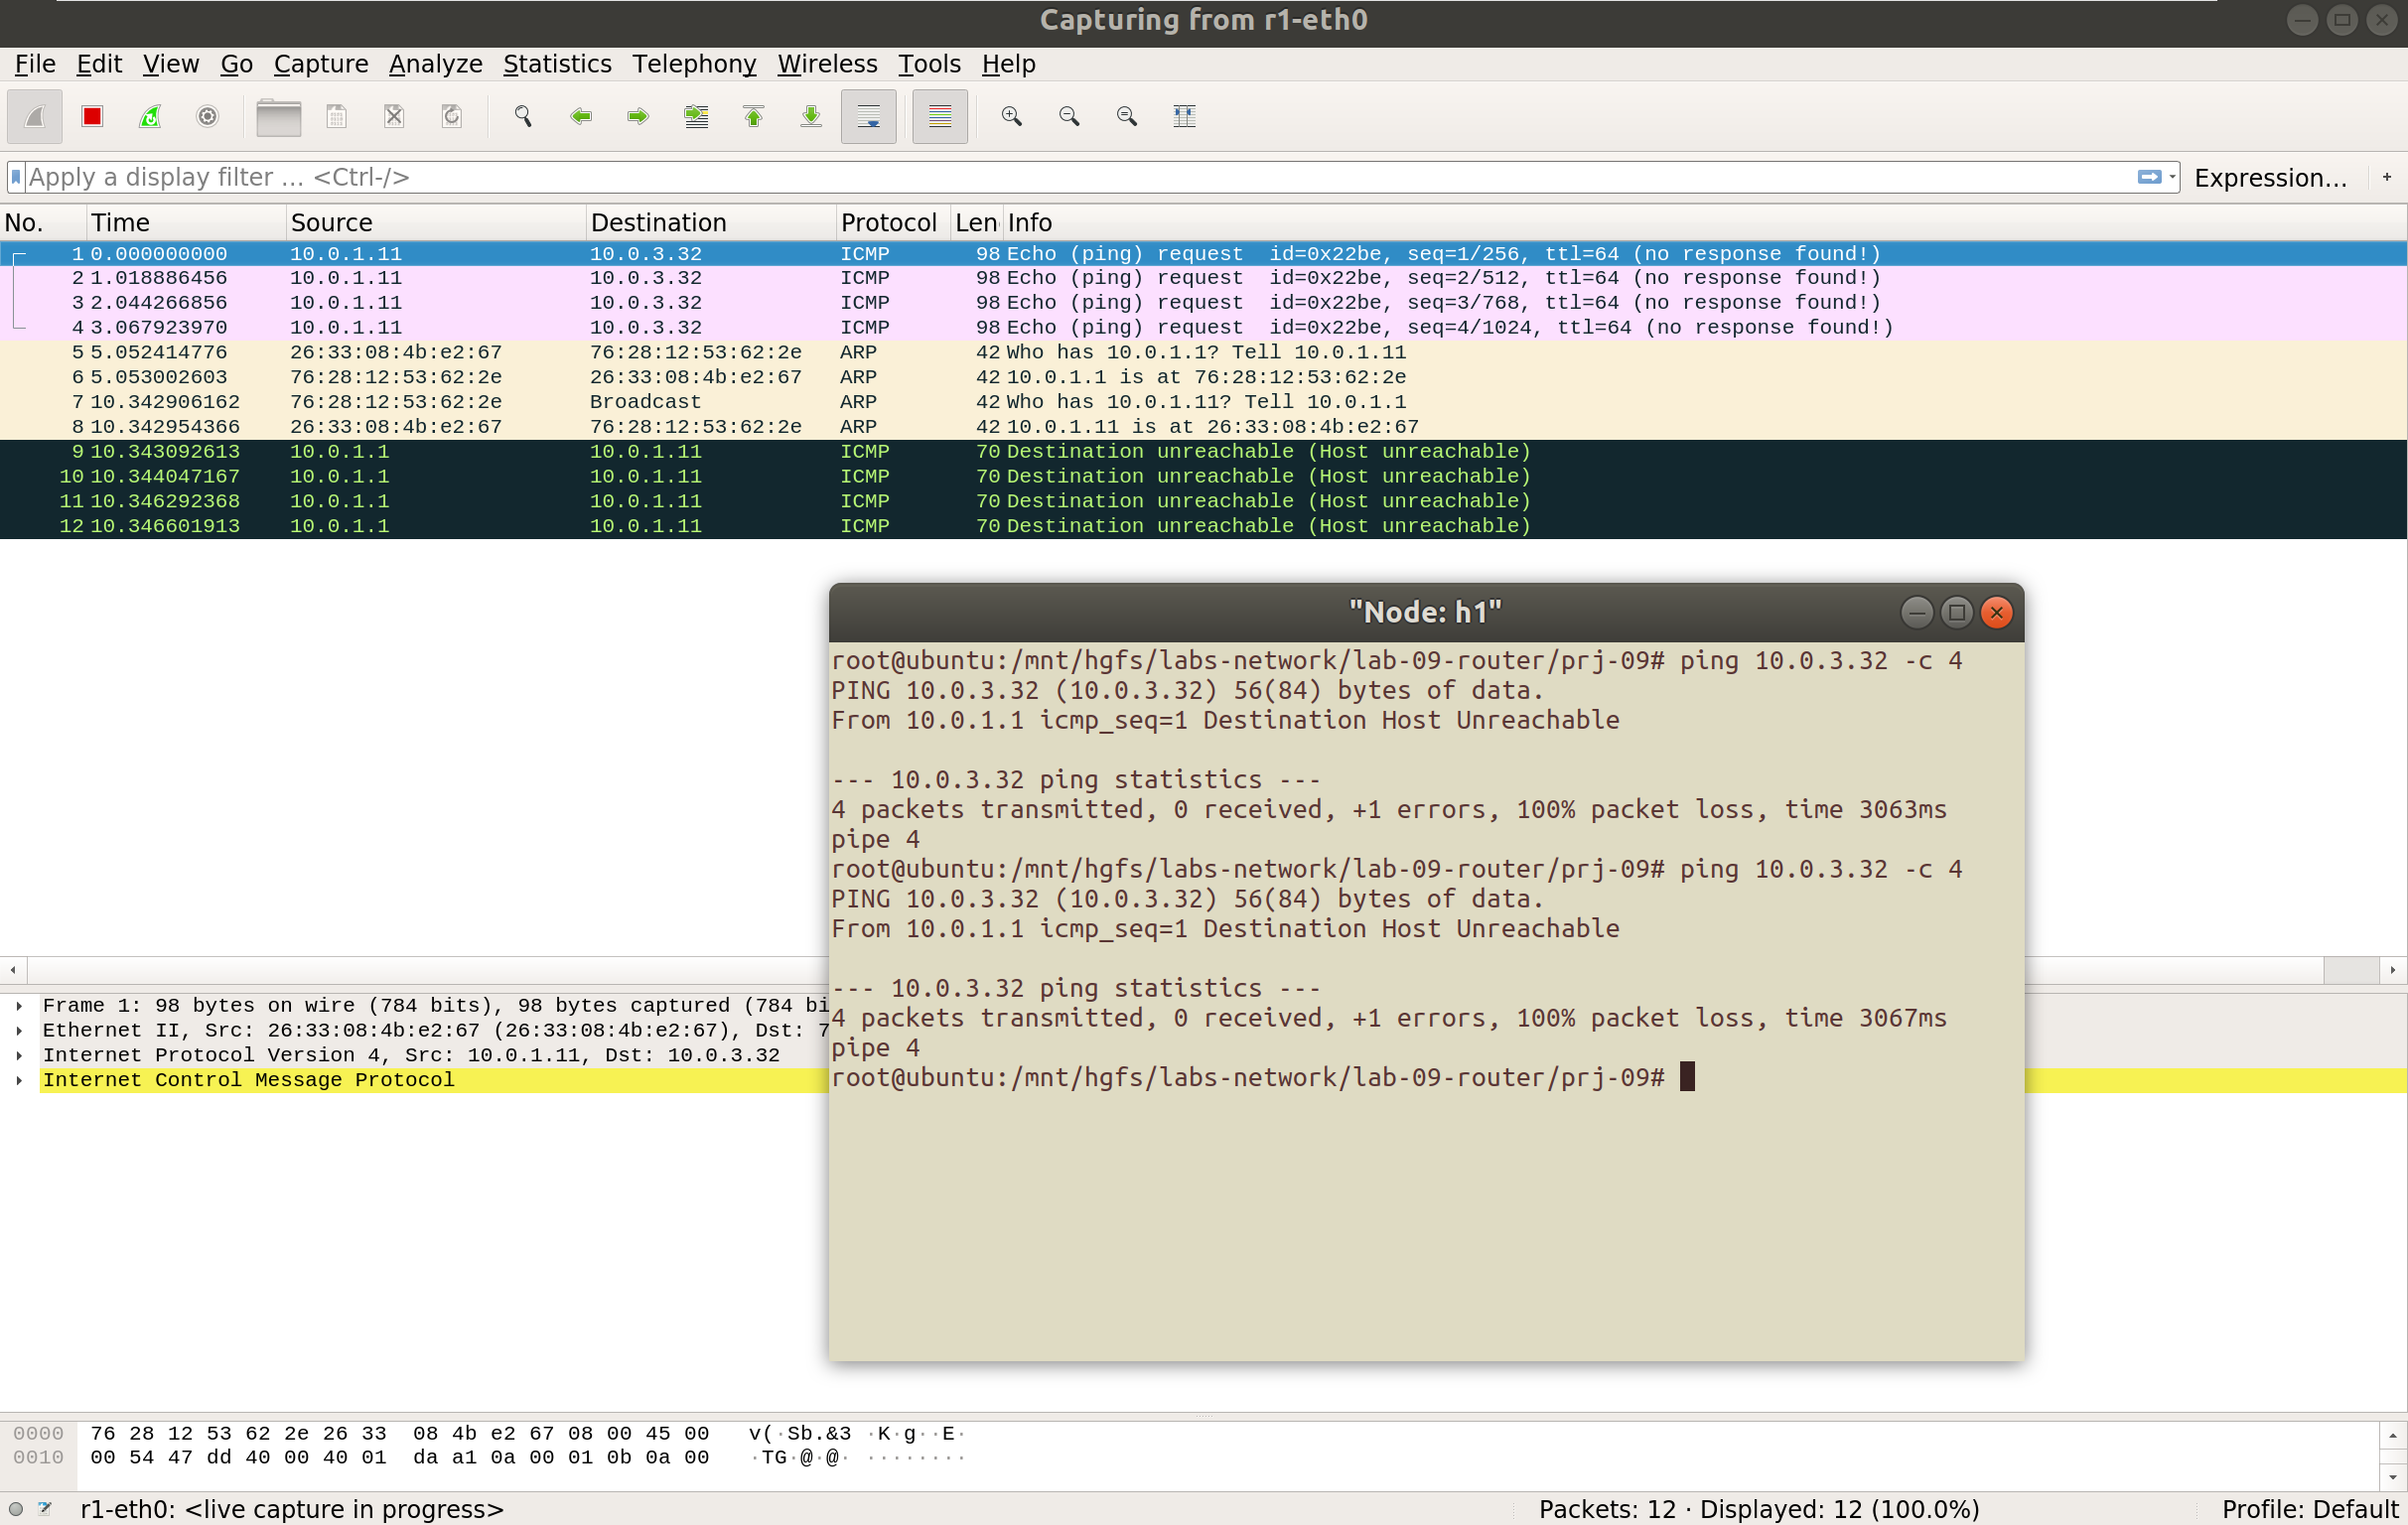
\includegraphics[width=230pt]{
                ../lab-09-router/readme.assets/burst-example.png}
            \caption{异常丢包: 发送无误, 接收有误} % 标题
        \end{figure}
    \end{block}
\end{frame}
\begin{frame}{程序的性能限制}{实验 9: 路由器转发实验}
    \begin{block}{分析与解决}
        \textbf{分析}:\\\quad 观察 ICMP消息的发送时间,
        发现相邻的消息之间发送时间差是毫秒级,
        据此猜测收包间隔过短可能影响端节点收包完整性.\\
        \textbf{解决}:\\\quad
        在 arp\_sweep 函数中发送 ICMP 消息的代码段之前加了一个
        'sleep(1)', 使程序挂起一段时间, 从而减小端节点的收包压力.\\
        \textbf{结果}:\\\quad
        重新编译后多次测试, 丢包现象不再出现.\\
        \textbf{结论}:\\\quad
        在我们的实验中 (虚拟网络环境+自己的程序),
        节点的收包能力有限, 发包间隔过短会使端节点来不及收包,
        进而产生丢包.
    \end{block}
\end{frame}


% 涉及的理论知识
\begin{frame}{涉及的理论知识}{实验 9: 路由器转发实验}
    该实验主要涉及路由器转发机制, 但并不要求我们实现路由表的生成和维护,
    只需要考虑 ARP Cache 的维护和根据路由表进行转发等.
\end{frame}

%%%%%%%%%%%%%%%%%%%%%%%%%%%%%%%%%%%%%%%%
%%%%%% 实验 10
\section{实验 10: 高效路由查找实验}
% 节标题
\begin{frame}
    \sectionpage
\end{frame}

% 实验过程
\begin{frame}{实验过程}{实验 10: 高效路由查找实验}
    \begin{block}{主要内容}
        1. 实现最基本的前缀树查找方案;\\
        2. 调研并实现某种 IP 前缀查找方案;\\
        3. 检查 IP 前缀查找的正确性, 测量所实现方案的性能.
    \end{block}
\end{frame}
\begin{frame}{Basic: Trie实现}{实验 10: 高效路由查找实验}
    \begin{block}{数据结构}
        统一internal node和match node的数据结构, 节点中含:\\
        1. 指向左孩子, 右孩子的结点指针\\
        2. 提示是否存有有效port信息的域match;\\
        3. 匹配的端口信息.
    \end{block}
\end{frame}
\begin{frame}{Advanced: PATRICIA Trie in FreeBSD}{实验 10: 高效路由查找实验}
    算法来源: Sklower K. A tree-based packet routing table
    for Berkeley unix[C]//USENIX Winter. 1991, 1991: 93-99.
    \begin{block}{数据结构}
        \textbf{中间结点}:\\
        \quad 1. 指向左孩子, 右孩子, 父母的结点指针;\\
        \quad 2. 提示是否为匹配节点的域match;\\
        \quad 3. 当下应比较的bit序号.\\
        \textbf{匹配结点}:\\
        \quad 1. 掩码, 端口, ip号;\\
        \quad 2. 提示是否为匹配节点的域match.
    \end{block}
    注: PATRICIA Tree是指radix=2的压缩前缀树(radix tree, 也称基数树)
\end{frame}
\begin{frame}{Advanced: PATRICIA Trie in FreeBSD}{实验 10: 高效路由查找实验}
    \begin{block}{示意图}
        \begin{figure}[h]
            \centering % 居中显示
            \includegraphics[width=200pt]{
                ../lab-10-lookup/readme.assets/routing_example.png}
            \caption{压缩前缀树算法的建树示意图} % 标题
        \end{figure}
    \end{block}
\end{frame}


% 实验结果展示
\begin{frame}{实验结果展示}{实验 10: 高效路由查找实验}\
    \begin{block}{建树/查找结果的正确性}
        在按数据集ip数据查找时, 输出与原数据集port信息的diff情况,
        发现两种算法的输出相同, 抽样检查后发现查找正确,
        即认为两种算法的正确性均得到保证.
    \end{block}
    \begin{block}{性能表现与内存占用比较}
        (以 basic 实现的测试结果为单位 "1")\\
        内存占用: 1 -> 0.03\% \\
        查找速度: 1 -> 1.56
    \end{block}
    虽然速度有所降低, 但大大减少了所需空间,
    因而该优化的效用是正的.
\end{frame}

% 涉及的理论知识
\begin{frame}{涉及的理论知识}{实验 10: 高效路由查找实验}
    该实验涉及路由表维护与查找的实际实现.
\end{frame}

%%%%%%%%%%%%%%%%%%%%%%%%%%%%%%%%%%%%%%%%
%%%%%% 实验 11
\section{实验 11: 网络路由实验}
% 节标题
\begin{frame}
    \sectionpage
\end{frame}

% 实验过程
\begin{frame}{实验过程}{实验 11: 网络路由实验}
    \begin{block}{主要内容}
        1. 基于已有代码框架,
        实现路由器生成和处理 mOSPF Hello/LSU 消息的相关操作,
        构建一致性链路状态数据库;\\
        2. 基于实验一, 实现路由器计算路由表项的相关操作.
    \end{block}
\end{frame}
\begin{frame}{实验过程}{实验 11: 网络路由实验}
    \begin{block}{构建一致性链路状态数据库}
        1. (端口) 收到 mospf hello 消息, 按需维护本端口的 nbr list ;\\
        2. (各端口) 定期发出包含端口信息的 mospf hello 消息;\\
        3. (路由器) 收到 mospf lsu 消息,
        按需更新路由器的链路状态数据库;\\
        4. (路由器从各个端口)
        定期发出包含所有端口的 nbr list 的 mospf lsu 消息;\\
        5. (各端口) 定期检查 nbr list 成员的时效性;\\
        6. (路由器) 定期检查链路状态数据库表项的时效性.
    \end{block}
    \begin{block}{路由表项的计算}
        1. 加载路由器列表, 将其映射为一张无负权的无向图;\\
        2. 将最短路径结果映射到路由, 更新路由表.
    \end{block}
\end{frame}

% 实验结果展示
\begin{frame}{实验结果展示}{实验 11: 网络路由实验}
    \begin{block}{test 1: 链路状态数据库生成}
        \begin{figure}[h]
            \centering % 居中显示
            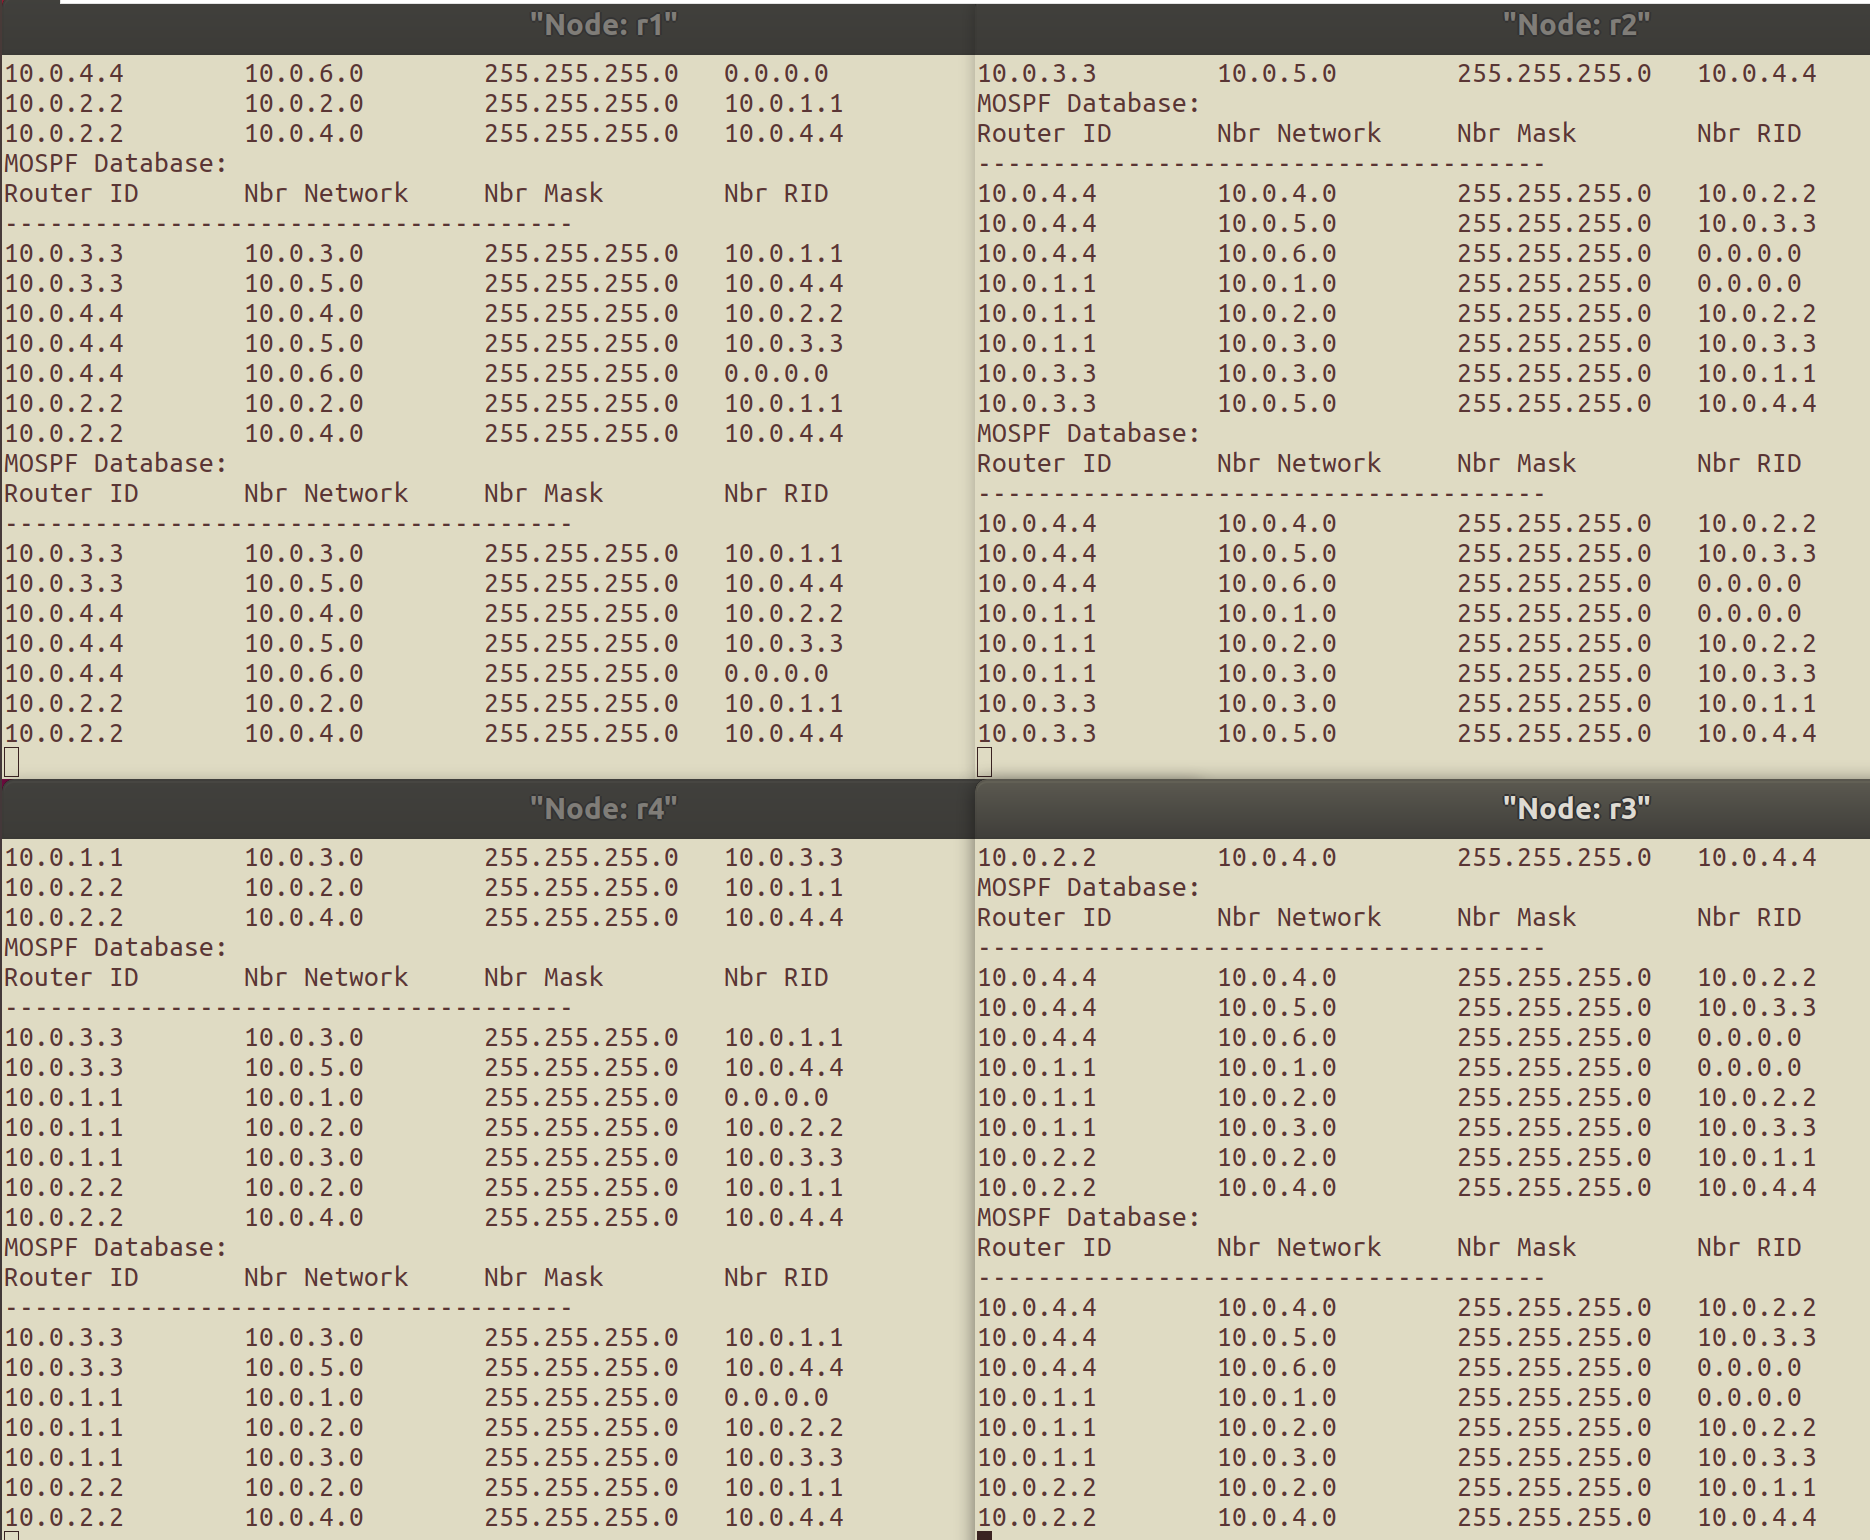
\includegraphics[width=190pt]{
                ../lab-11-mospf/readme.assets/p1-result.png}
            \caption{各节点的链路状态数据库} % 标题
        \end{figure}
    \end{block}
\end{frame}
\begin{frame}{实验结果展示}{实验 11: 网络路由实验}
    \begin{block}{test 2: 路由表项计算}
        \begin{figure}[h]
            \centering % 居中显示
            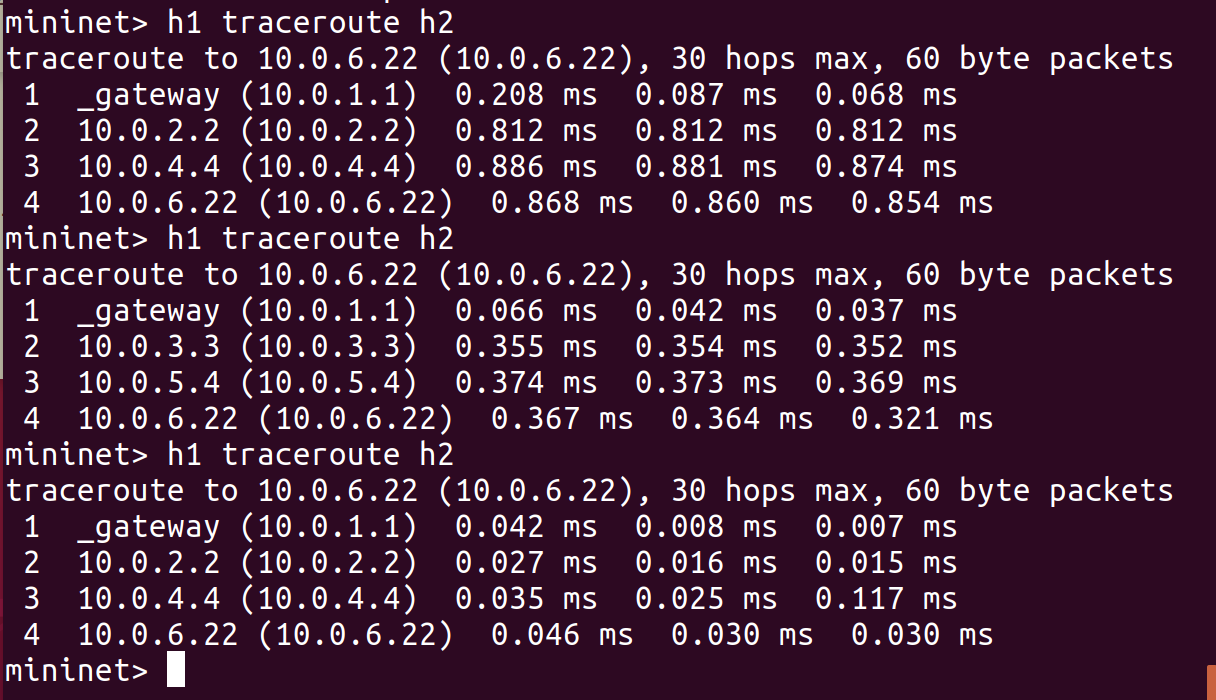
\includegraphics[width=180pt]{
                ../lab-11-mospf/readme.assets/p2-shut-node-r2.png}
            \caption{
                路由表项计算: 完整拓扑 -> 删去节点(r2) -> 恢复节点} % 标题
        \end{figure}
    \end{block}
\end{frame}
\begin{frame}{实验结果展示}{实验 11: 网络路由实验}
    \begin{block}{test 2: 路由表项计算}
        \begin{figure}[h]
            \centering % 居中显示
            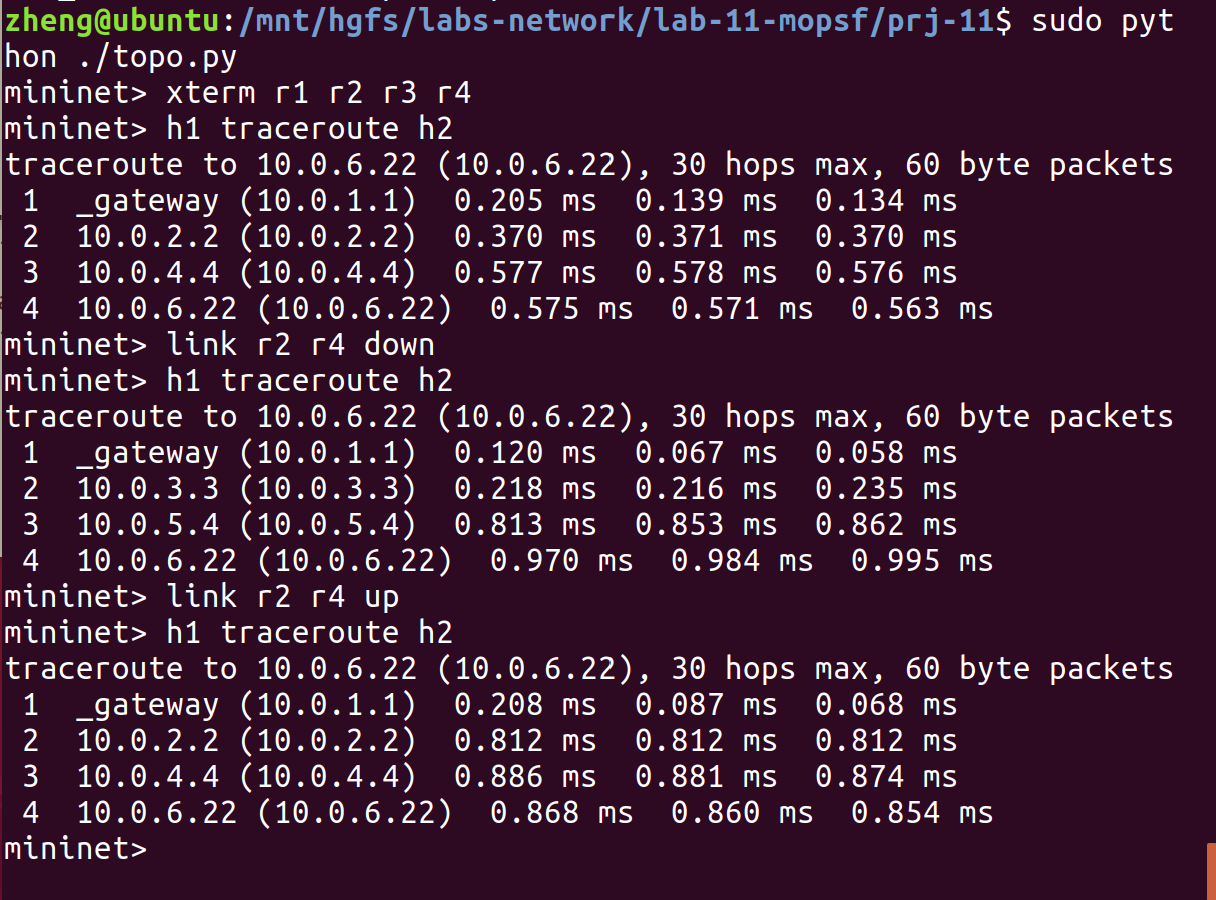
\includegraphics[width=180pt]{
                ../lab-11-mospf/readme.assets/p2-shut-link-r2-to-r4.png}
            \caption{
                路由表项计算: 完整拓扑 -> 删去链路(r2-r4) -> 恢复链路} % 标题
        \end{figure}
    \end{block}
\end{frame}

% 实验反思
\begin{frame}{实验反思}{实验 11: 网络路由实验}
    \begin{block}{遇到的问题}
        traceroute 时, icmp 消息回传不一定通过路由路径的端口,
        只能保证途经端口属于响应的途径路由器.
    \end{block}
    \begin{block}{分析与解决}
        回传时 icmp send packet 是通过本地路由来决定回传端口的,
        这说明各节点路由表的计算出现了不一致.\\
        经过排查, 发现原因: 将路由器节点映射为图节点时,
        没有考虑为路由表中的节点赋予统一的顺序 (如升序),
        导致计算的路由并不是一致的.\\
        在生成图节点列表时加上排序的步骤即可.
    \end{block}
\end{frame}

% 涉及的理论知识
\begin{frame}{涉及的理论知识}{实验 11: 网络路由实验}
    该实验内容是 OSPF 协议的简化版.
    通过该实验, 我们了解了该协议如何通过ospf hello 和 ospf lsu
    消息在各个路由器节点上动态地维护一致的链路状态数据库.
\end{frame}

%%%%%%%%%%%%%%%%%%%%%%%%%%%%%%%%%%%%%%%%
%%%%%% 实验 12
\section{实验 12: 网络地址转换实验}
% 节标题
\begin{frame}
    \sectionpage
\end{frame}

% 实验过程
\begin{frame}{实验过程}{实验 12: 网络地址转换实验}
    \begin{block}{主要内容}
        1. SNAT 实现;\\
        2. DNAT 实现;\\
        3. 在1-2的基础上验证双 NAT 可行.
    \end{block}

    \begin{block}{实验流程}
        0. 解析 conf 文件, 载入NAT rule;\\
        1. 确定pkt方向 (IN/OUT);\\
        2. 根据NAT rule 重写并发包 or
        添加连接 or 发送主机不可达;\\
        3. NAT连接定时老化;\\
        4. NAT释放.
    \end{block}
\end{frame}

% 实验结果展示
\begin{frame}{验证DNAT}{实验 12: 网络地址转换实验}
    \begin{figure}[h]
        \centering % 居中显示
        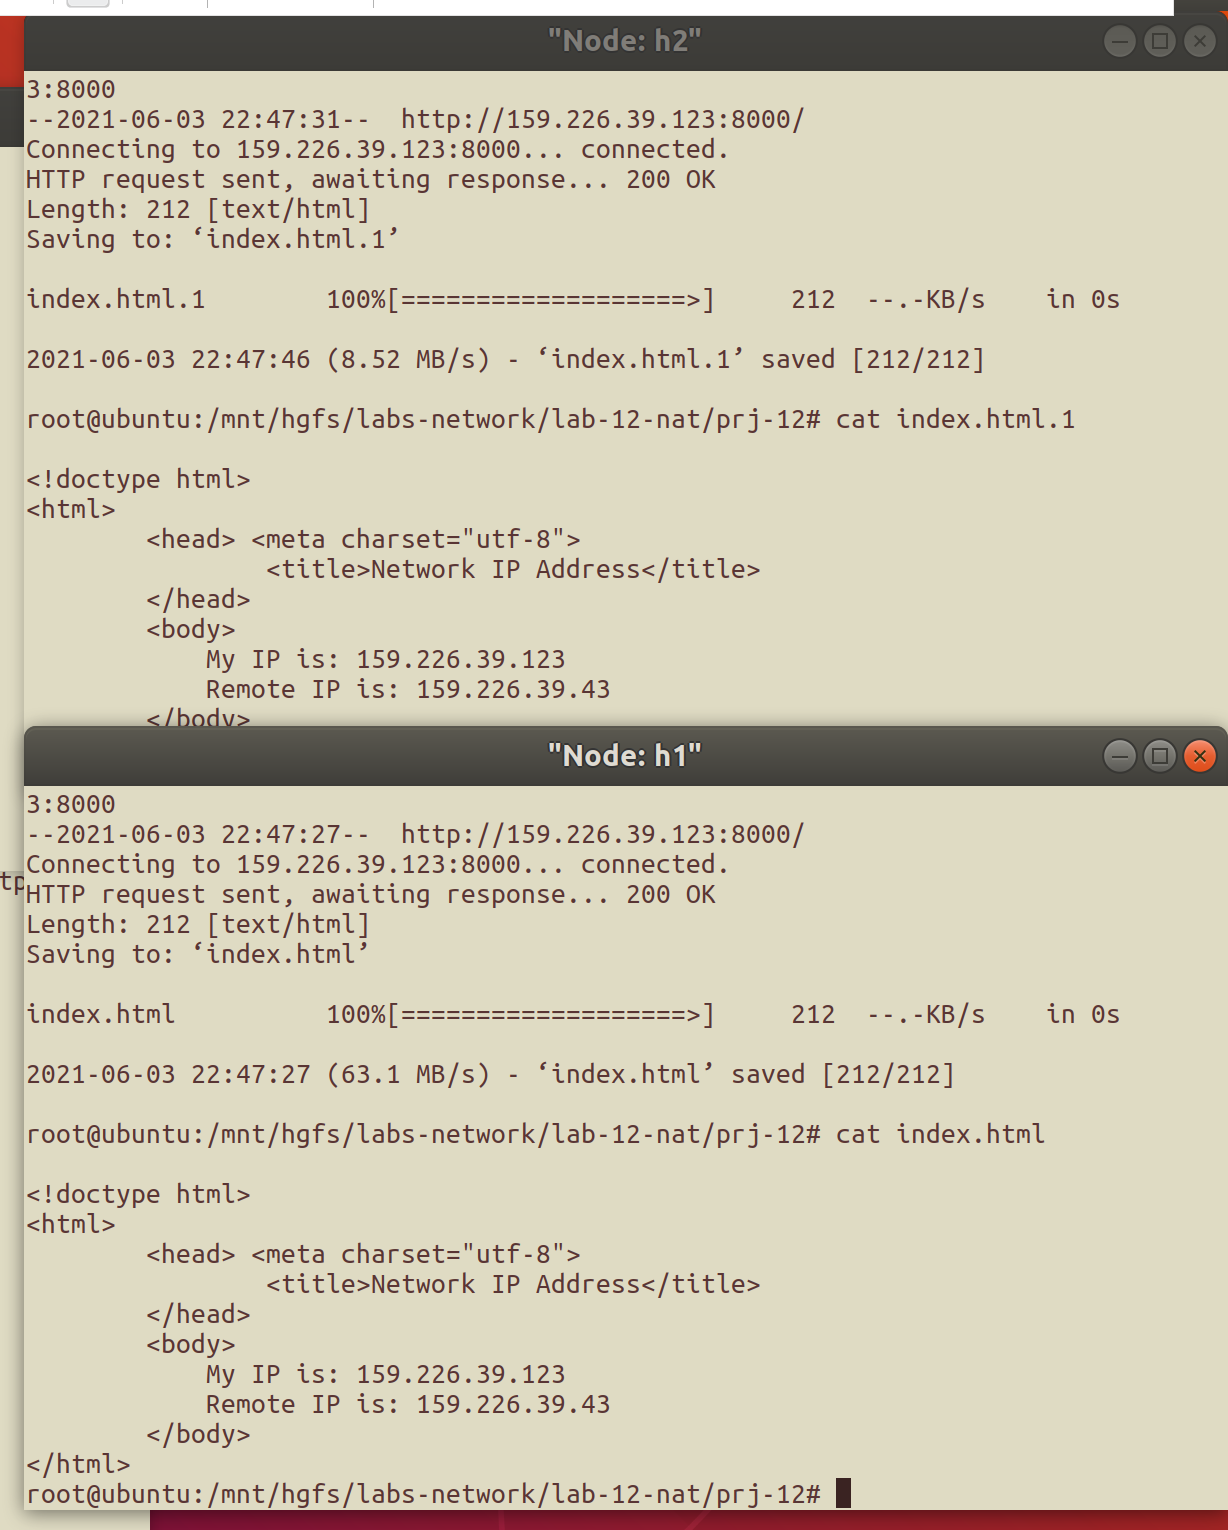
\includegraphics[width=160pt]{
            ../lab-12-nat/readme.assets/p1-website.png}
        \caption{验证DNAT (shell)} % 标题
    \end{figure}
\end{frame}
\begin{frame}{验证DNAT}{实验 12: 网络地址转换实验}
    \begin{figure}[h]
        \centering % 居中显示
        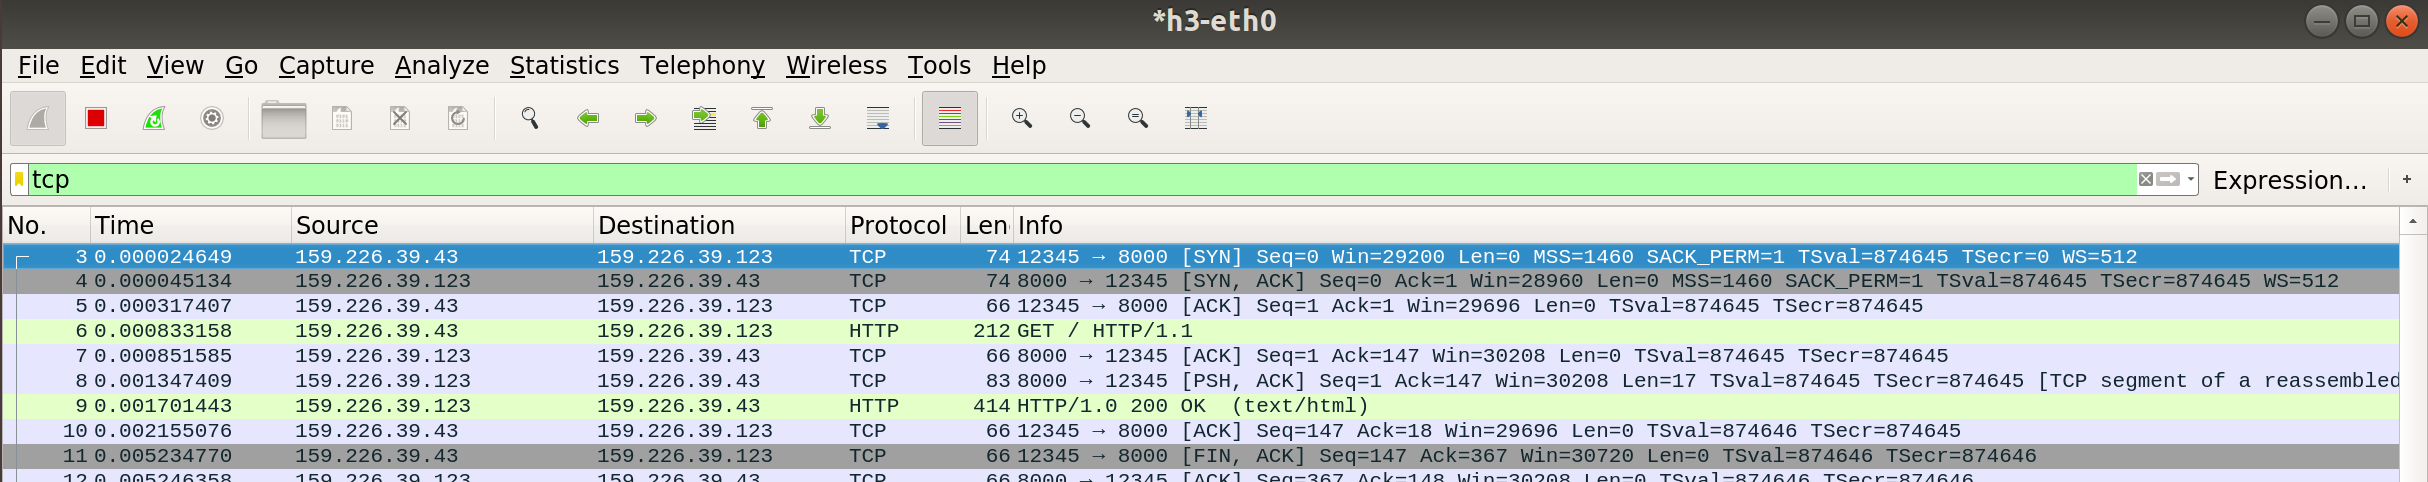
\includegraphics[width=300pt]{
            ../lab-12-nat/readme.assets/p1-ws.png}
        \caption{验证DNAT (wireshark)} % 标题
    \end{figure}
\end{frame}
\begin{frame}{验证SNAT}{实验 12: 网络地址转换实验}
    \begin{figure}[h]
        \centering % 居中显示
        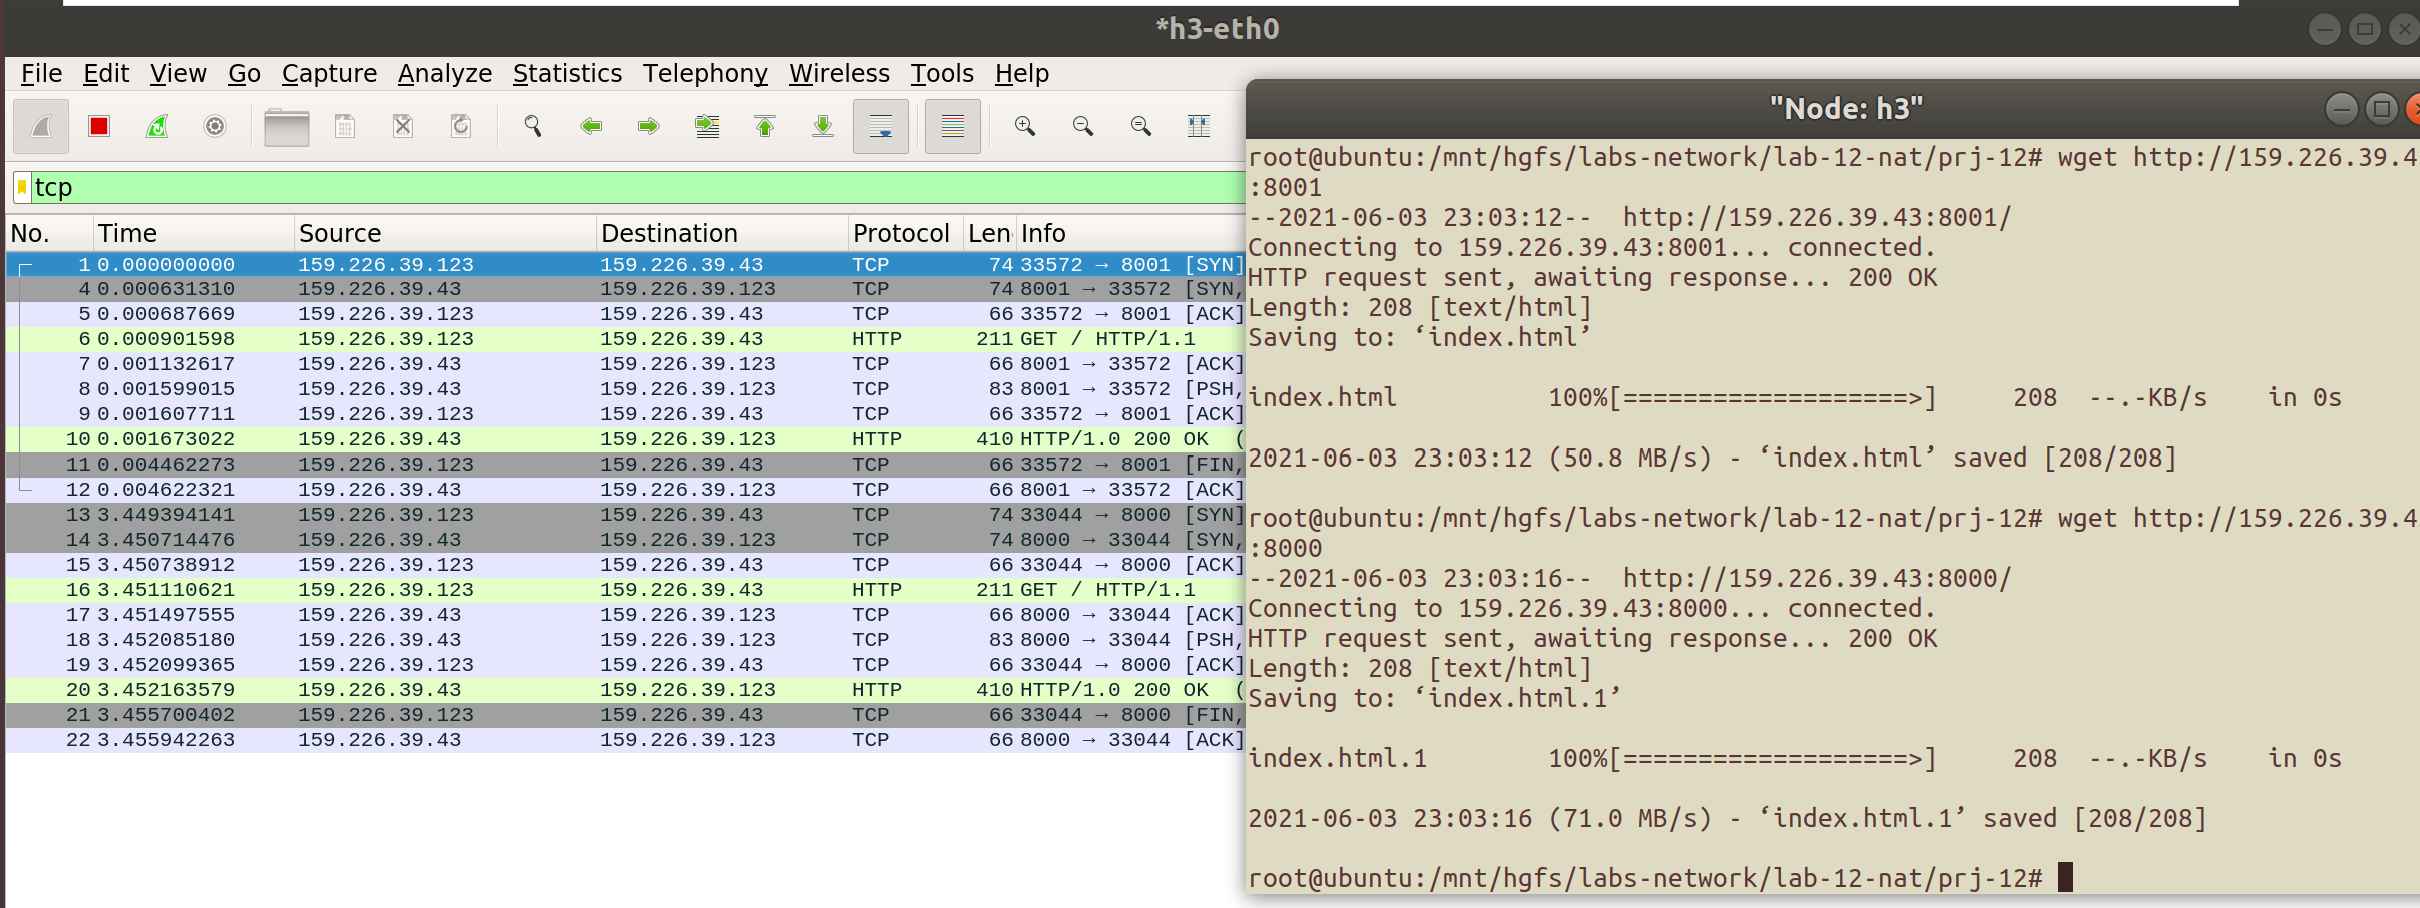
\includegraphics[width=300pt]{
            ../lab-12-nat/readme.assets/p2.png}
        \caption{验证SNAT (shell+wireshark)} % 标题
    \end{figure}
\end{frame}
\begin{frame}{验证双NAT}{实验 12: 网络地址转换实验}
    拓扑: h1 - n1 - n2 - h2
    \begin{figure}[h]
        \centering % 居中显示
        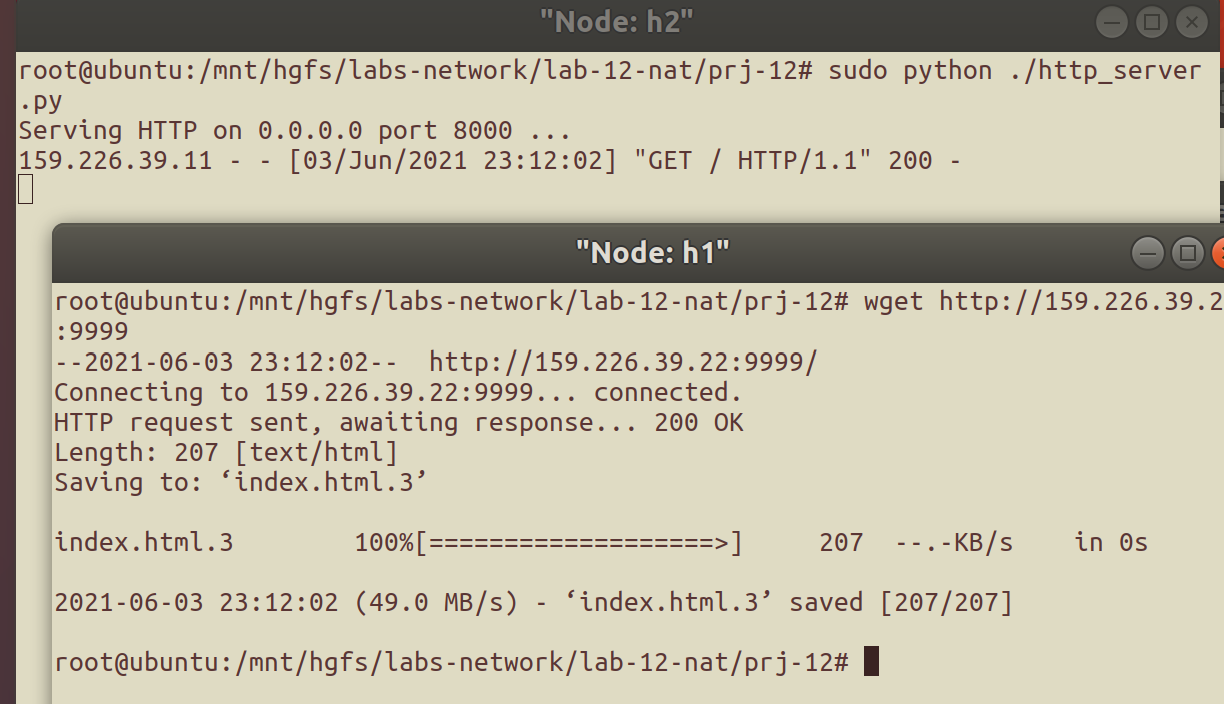
\includegraphics[width=200pt]{
            ../lab-12-nat/readme.assets/p3-a.png}
        \caption{验证双NAT: h1 请求 h2} % 标题
    \end{figure}
\end{frame}
\begin{frame}{验证双NAT}{实验 12: 网络地址转换实验}
    拓扑: h1 - n1 - n2 - h2
    \begin{figure}[h]
        \centering % 居中显示
        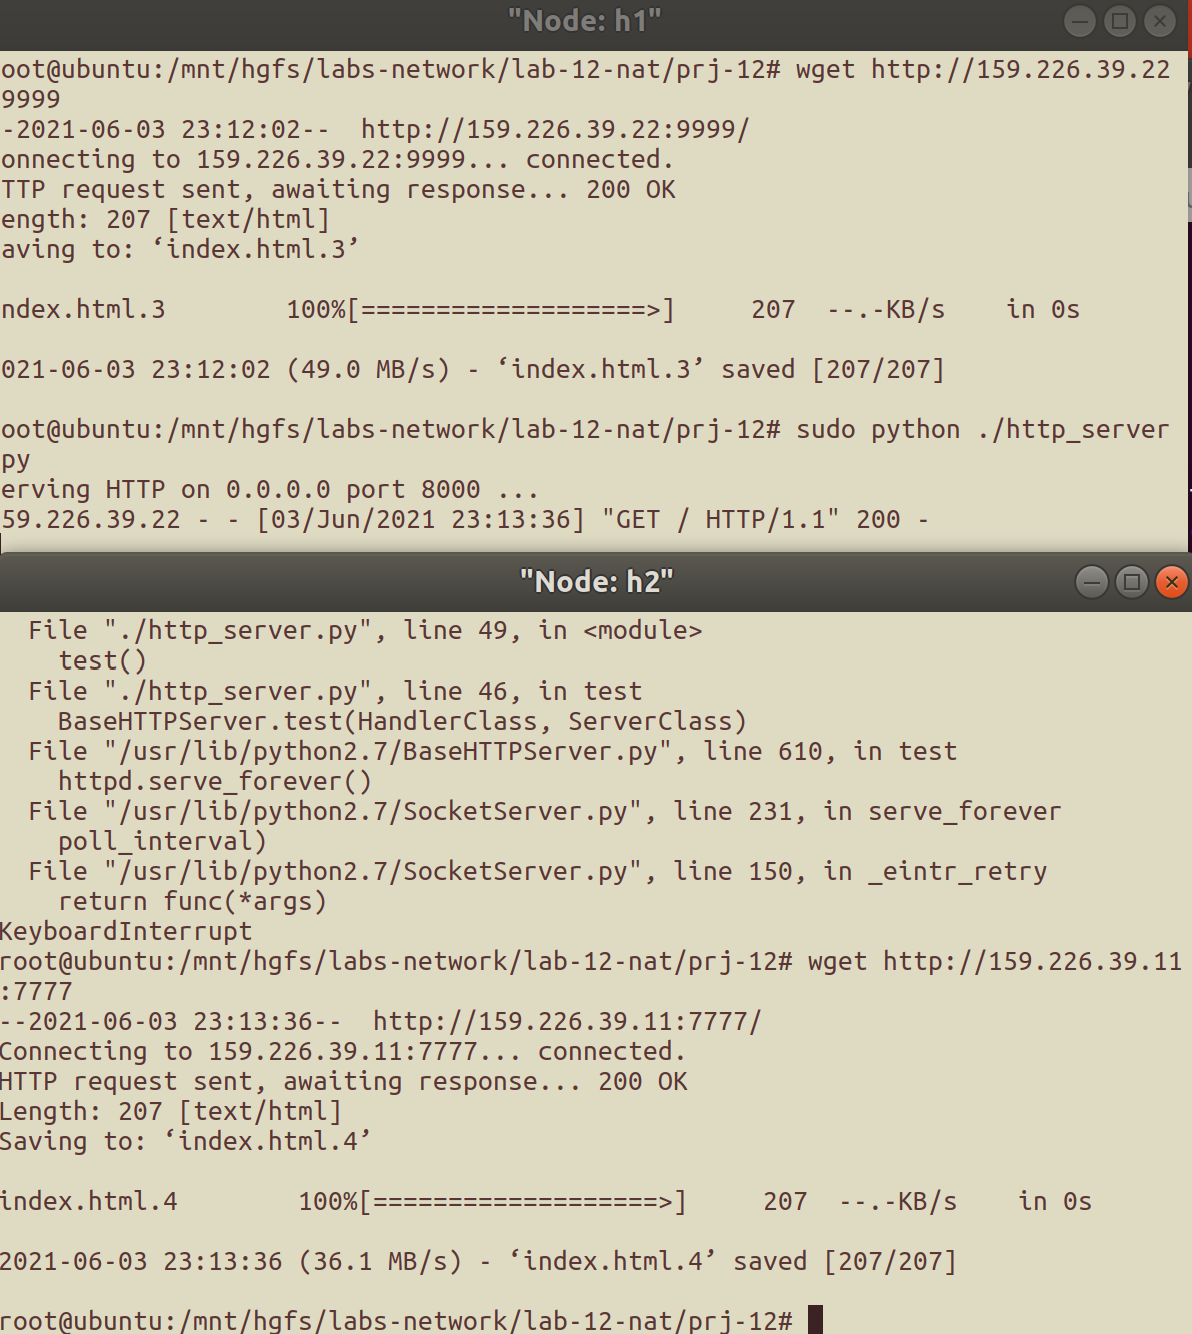
\includegraphics[width=150pt]{
            ../lab-12-nat/readme.assets/p3-b.png}
        \caption{验证双NAT: h2 请求 h1} % 标题
    \end{figure}
\end{frame}

% 涉及的理论知识
\begin{frame}{涉及的理论知识}{实验 12: 网络地址转换实验}
    NAT提供了一种地址转换方法, 使私网主机能在不暴露自己真实地址的同时与其他主机交互, 并且由于该方法的核心是端口/地址的映射, 从而支持多层 NAT的存在.
\end{frame}

%%%%%%%%%%%%%%%%%%%%%%%%%%%%%%%%%%%%%%%%
% 可用元素

%% 实验总结小模板

% %%%%%%%%%%%%%%%%%%%%%%%%%%%%%%%%%%%%%%%%
% %%%%%% 实验 x
% \section{实验 x: xxxxxx}
% % 节标题
% \begin{frame}
%     \sectionpage
% \end{frame}

% % 实验过程
% \begin{frame}{实验过程}{}
%     \begin{block}{主要内容}
%     \end{block}

%     \begin{block}{实验流程}
%     \end{block}
% \end{frame}

% % 实验结果展示
% \begin{frame}{实验结果展示}{}
% \end{frame}

% % 实验反思
% \begin{frame}{实验反思}{}
%     \begin{block}{实验心得}
%     \end{block}

%     \begin{block}{遇到的问题}
%     \end{block}
% \end{frame}
%
% % 涉及的理论知识
% \begin{frame}{涉及的理论知识}{}
% \end{frame}

\end{document}
